%% This is file `DEMO-TUDaThesis.tex' version 3.32 (2023/06/19),
%% it is part of
%% TUDa-CI -- Corporate Design for TU Darmstadt
%% ----------------------------------------------------------------------------
%%
%%  Copyright (C) 2018--2023 by Marei Peischl <marei@peitex.de>
%%
%% ============================================================================
%% This work may be distributed and/or modified under the
%% conditions of the LaTeX Project Public License, either version 1.3c
%% of this license or (at your option) any later version.
%% The latest version of this license is in
%% http://www.latex-project.org/lppl.txt
%% and version 1.3c or later is part of all distributions of LaTeX
%% version 2008/05/04 or later.
%%
%% This work has the LPPL maintenance status `maintained'.
%%
%% The Current Maintainers of this work are
%%   Marei Peischl <tuda-ci@peitex.de>
%%   Markus Lazanowski <latex@ce.tu-darmstadt.de>
%%
%% The development respository can be found at
%% https://github.com/tudace/tuda_latex_templates
%% Please use the issue tracker for feedback!
%%
%% If you need a compiled version of this document, have a look at
%% http://mirror.ctan.org/macros/latex/contrib/tuda-ci/doc
%% or at the documentation directory of this package (if installed)
%% <path to your LaTeX distribution>/doc/latex/tuda-ci
%% ============================================================================
%%
% !TeX program = lualatex
%%

\documentclass[
	english, % was: ngerman,
	ruledheaders=section,%Ebene bis zu der die Überschriften mit Linien abgetrennt werden, vgl. DEMO-TUDaPub
	class=report,% Basisdokumentenklasse. Wählt die Korrespondierende KOMA-Script Klasse
	thesis={type=bachelor},% Dokumententyp Thesis, für Dissertationen siehe die Demo-Datei DEMO-TUDaPhd
	accentcolor=9c,% Auswahl der Akzentfarbe
	custommargins=false,%true,% Ränder werden mithilfe von typearea automatisch berechnet
	marginpar=false,% Kopfzeile und Fußzeile erstrecken sich nicht über die Randnotizspalte
	%BCOR=5mm,%Bindekorrektur, falls notwendig
	parskip=half-,%Absatzkennzeichnung durch Abstand vgl. KOMA-Script
	fontsize=11pt,%Basisschriftgröße laut Corporate Design ist mit 9pt häufig zu klein
	instbox=true,
    oneside,% TODO: only change to 'twoside' for printing (enables \cleardoublepage)
	% logofile=Graphics/tuda_logo.pdf, %Falls die Logo Dateien nicht vorliegen
]{tudapub}


% Der folgende Block ist nur bei pdfTeX auf Versionen vor April 2018 notwendig
\usepackage{iftex}
\ifPDFTeX
	\usepackage[utf8]{inputenc}%kompatibilität mit TeX Versionen vor April 2018
\fi

%%%%%%%%%%%%%%%%%%%
%Sprachanpassung & Verbesserte Trennregeln
%%%%%%%%%%%%%%%%%%%
\usepackage[main=english]{babel} % was: [english, main=ngerman]{babel}
\usepackage[autostyle]{csquotes}% Anführungszeichen vereinfacht

% Falls mit pdflatex kompiliert wird, wird microtype automatisch geladen, in diesem Fall muss diese Zeile entfernt werden, und falls weiter Optionen hinzugefügt werden sollen, muss dies über
% \PassOptionsToPackage{Optionen}{microtype}
% vor \documentclass hinzugefügt werden.
\usepackage{microtype}
%%%%%%%%%%%%%%%%%%%
%Literaturverzeichnis
%%%%%%%%%%%%%%%%%%%
\usepackage{biblatex}   % Literaturverzeichnis
\bibliography{meta/references.bib}


%%%%%%%%%%%%%%%%%%%
%Paketvorschläge Tabellen
%%%%%%%%%%%%%%%%%%%
%\usepackage{array}     % Basispaket für Tabellenkonfiguration, wird von den folgenden automatisch geladen
\usepackage{tabularx}   % Tabellen, die sich automatisch der Breite anpassen
%\usepackage{longtable} % Mehrseitige Tabellen
%\usepackage{xltabular} % Mehrseitige Tabellen mit anpassbarer Breite
\usepackage{booktabs}   % Verbesserte Möglichkeiten für Tabellenlayout über horizontale Linien
% weitere
\usepackage{multirow}

%%%%%%%%%%%%%%%%%%%
%Paketvorschläge Mathematik
%%%%%%%%%%%%%%%%%%%
% Vorschläge Damken
%\usepackage{amsmath}
%\usepackage{amssymb}
%\usepackage[mathscr]{eucal}
% Vorschläge TUDA
\usepackage{mathtools} % erweiterte Fassung von amsmath
\usepackage{amssymb}   % erweiterter Zeichensatz
\usepackage{siunitx}   % Einheiten

%%%%%%%%%%%%%%%%%%%
% weitere eigne
%%%%%%%%%%%%%%%%%%%
\usepackage{xcolor,colortbl}    % Farben, Tabellenfarben
\definecolor{BG}{gray}{0.85}    % Background color used for tables
\usepackage{float}              % place tables manually by using [H] (not only [h] or [h!]), working nice :)

%%%%%%%%%%%%%%%%%%
% make nice Trees
% from: https://tex.stackexchange.com/questions/23647/drawing-a-directory-listing-a-la-the-tree-command-in-tikz
% and: https://texample.net/tikz/examples/filesystem-tree/
%%%%%%%%%%%%%%%%%
\usepackage{tikz}               % Trees
\makeatletter
\newcount\dirtree@lvl
\newcount\dirtree@plvl
\newcount\dirtree@clvl
\def\dirtree@growth{%
  \ifnum\tikznumberofcurrentchild=1\relax
  \global\advance\dirtree@plvl by 1
  \expandafter\xdef\csname dirtree@p@\the\dirtree@plvl\endcsname{\the\dirtree@lvl}
  \fi
  \global\advance\dirtree@lvl by 1\relax
  \dirtree@clvl=\dirtree@lvl
  \advance\dirtree@clvl by -\csname dirtree@p@\the\dirtree@plvl\endcsname
  \pgf@xa=0.35cm\relax      % length of horizontal line   % was 1cm\relax
  \pgf@ya=-0.7cm\relax      % distances between child-nodes % was -1cm\relax,  -0.7 is more compact, without overlaping
  \pgf@ya=\dirtree@clvl\pgf@ya
  %\pgf@xa=\dirtree@plvl\pgf@xa  % this does do something .... but not, what I want ...
  \pgftransformshift{\pgfqpoint{\the\pgf@xa}{\the\pgf@ya}} % shifte x, y but only relative to parents center ...
  % was {\the\pgf@xa}{\the\pgf@ya}} ... you should be able to shift here ...
  \ifnum\tikznumberofcurrentchild=\tikznumberofchildren
  \global\advance\dirtree@plvl by -1
  \fi
}

\tikzset{
  dirtree/.style={
    growth function=\dirtree@growth,
    every node/.style={draw=black,thick,anchor=north},
    every child node/.style={draw=black,thick,anchor=west},
    edge from parent path={(\tikzparentnode\tikzparentanchor) |- (\tikzchildnode\tikzchildanchor)}
  }
}
\makeatother

%%%%%%%%%%%%%%%%%%
% make colored operators
% from: https://tex.stackexchange.com/questions/273941/how-to-change-color-of-operators-lim-log-etc
%%%%%%%%%%%%%%%%%
%\usepackage{xcolor,amsmath
\usepackage{xpatch,letltxmacro}
% \DeclareMathOperator{\abc}{abc}                    % just new math operator
% \xpatchcmd{\qopname}{#3}{\textcolor{red}{#3}}{}{}  % all min, max, sin, etc --> red 
\LetLtxMacro\latexsqrt\sqrt
\NewDocumentCommand{\sqrtRed}{om}{       % was: \RenewDocumentCommand{\sqrt}{om}{%
  \colorlet{current}{.}
  \IfNoValueTF{#1}
    {\textcolor{red}{\latexsqrt{\textcolor{current}{#2}}}}%
    {\textcolor{red}{\latexsqrt[#1]{\textcolor{current}{#2}}}}%
}

%% use:
  % \sqrtRed{blabla}
  %% was:
  % \abc d \quad
  % \sin \theta \quad
  % \log_e \quad
  % \lim_{x \rightarrow 0} \quad
  % \int_a^b \quad
  % \sqrt{2} \quad
  % \sqrt[3]{x+1}

\setcounter{secnumdepth}{3}     % so \autoref also will show 3ed lvl like 03.2.1.1 not only 03.2.1

%Formatierungen für Beispiele in diesem Dokument. Im Allgemeinen nicht notwendig!
%\let\file\texttt
%\let\code\texttt
%\let\tbs\textbackslash
%\let\pck\textsf
%\let\cls\textsf

\usepackage{pifont}% Zapf-Dingbats Symbole
\newcommand*{\FeatureTrue}{\ding{52}}
\newcommand*{\FeatureFalse}{\ding{56}}

\newcommand{\todo}[1]{{\color{blue}\textbf{TODO: } #1\textbf{}}\newline}
\newcommand{\note}[1]{{\color{red}\textbf{note: } #1\textbf{}}} % or with \newline}
\newcommand{\atJohn}[1]{{\color{violet}\textbf{@ John: } #1\textbf{}}} % or with \newline}
\newcommand{\bgA}[1]{{}\colorbox{gray}{}}  %background for tabels


%%% toogle tables in text %%%
\newif\iftable
\tablefalse % set true / false here
%%% %%%
\begin{document}

\Metadata{
	title=Dataset Balancing for Improving Robustness of Medical Neural Cellular Automata,  % TODO: adjust title
	author=R. Spari,
}

\title{Improving Robustness of Neural Cellular Automata for Medical Image Segmentation with a Variance Based Quality Metric}  % TODO: adjust title
%\subtitle{\color{red} Subtitel}
\author[R.Spari]{Ruben Spari} %optionales Argument ist die Signatur,
\birthplace{Limburg, Deutschland}
\reviewer{  % TODO: adjust reviewers
	Anirban Mukhopadhyay
	\and
	John Kalkhof
	% \and
	% \color{red} maybe somebody else
}

%Diese Felder werden untereinander auf der Titelseite platziert.
%\department ist eine notwendige Angabe, siehe auch dem Abschnitt `Abweichung von den Vorgaben für die Titelseite'
\department{inf} % Das Kürzel wird automatisch ersetzt und als Studienfach gewählt, siehe Liste der Kürzel im Dokument.
\institute{Interactive Graphics Systems Group}
\group{Medical and Environmental Computing}
\addTitleBoxLogo*{
\includegraphics[width=1.0\linewidth]{Graphics/GRIS+MecLabLogo.png}}  % was width=0.75 % TODO: adjust group logo; you might want to set instbox=false

\submissiondate{\today}
\examdate{\today}

% Hinweis zur Lizenz:
% TUDa-CI verwendet momentan die Lizenz CC BY-NC-ND 2.0 DE als Voreinstellung.
% Die TU Darmstadt hat jedoch die Empfehlung von dieser auf die liberalere
% CC BY 4.0 geändert. Diese erlaubt eine Verwendung bearbeiteter Versionen und
% die kommerzielle Nutzung.
% TUDa-CI wird im nächsten größeren Release ebenfalls diese Anpassung vornehmen.
% Aus diesem Grund wird empfohlen die Lizenz manuell auszuwählen.
%\tuprints{urn=XXXXX,printid=XXXX,year=2022,license=cc-by-4.0}
% To see further information on the license option in English, remove the license= key and pay attention to the warning & help message.

% \dedication{Für alle, die \TeX{} nutzen.}

% TODO ???: can use 	\pagenumbering{gobble} ... 	\pagenumbering{Roman}  % I, II, … ... 	\pagenumbering{arabic}  % 1, 2, … like is Fabian Darmken to use diffrent sets of pagenumbers for pre-content stuff. But will start with page number "1" on first content page. So you hae like 4 pages less ...

\pagenumbering{gobble}                        % or include againe ?
{
    \maketitle
}

\cleardoublepage
\pagenumbering{Roman}  % I, II, …             % or include againe ?
{
    \begin{abstract}
% Teil #1 – Worum geht es?                       = Fragestellung 
%                                                = 1. Die Erklärung der Problemstellung 
%                                                = die Fragestellung und generelle Zielsetzung deiner Abschlussarbeit
Neural Cellular Automatas (NCAs) are a promising deep-learning approach for medical image segmentation because they are lightweight while producing high-quality segmentations. They can be used in many environments where the prevailing large-scale segmentation models, primarily based on U-Nets, are too large because the resources are unavailable, as with many primary care facilities, due to economic or general local developments or crises. Like other machine learning models, NCAs, too, can suffer from performance degradation when confronted with perturbations in the data or domain shifts (out of distribution data). However, in critical scenarios, like medical imaging, where people's health is at stake, robustness against such disruptions is of crucial importance. This thesis presents an approach to improve the robustness of NCAs for medical image segmentation against such perturbations based on the NCA Quality Score (NQM), a variance-based quality metric.


% Teil #2 – Wie hast du das Thema bearbeitet?    = Methoden      
%                                                = 2. Inwiefern der Ansatz anders ist zu bestehenden und was die Intuition ist 
%                                                = Welche Methodik wurde wie angewendet? 
%                                                = Hypothesen und verwendete Methoden
Unlike most neural networks, the output of NCAs is not deterministic but stochastic. Therefore, different outputs are generated for the same input each time. The NQM is a scalar metric based on the variance of these outputs and has been used to indicate the stability of the model and detect failure cases. We propose to utilize the variance captured in the NQM metric for training by including it in the loss function. Our experiments take a broad exploratory approach. We developed several loss functions in which we adapted the NQM. First of all, one, where it is weighted linearly. We simulated various disturbances in datasets to test these losses for robustness. On the one hand, we used different augmentations to simulate radiological noise, and on the other hand, mixing datasets from different sources but from the same organ to simulate domain shifts.
To speed up training, further increase robustness, and improve stability, we also performed tests on pre-trained models, investigated two hyperparameters, developed three non-linear losses, and compared them with the linear variant in different sub-variants.


% Teil #3 – Was sind die wichtigsten Ergebnisse? = Ergebnisse    
%                                                = 3. Was genau damit erreicht wurde, insgesamt, mit Präsentation der Ergebnisse 
%                                                = Was sind die wichtigsten Ergebnisse?
Our approach improves the robustness of NCAs against radiological perturbations by up to 15 points on the Dice. Especially with pretrained models and adjustments to the hyperparameters, we were able to develop a fast and stable method. Some non-linear variants show equally stable behavior, while others perform relatively poorly. We assume that the stable ones can further improve our method. For domain shifts with single or few out-of-domain samples, there are shifts in performance. Some models perform better, others worse. We assume the challenging dataset is a significant factor.


Overall, our results clearly show that integrating the NQM into the loss is a powerful tool to improve the robustness of NCAs for medical image segmentation.


%%% Keywords %%%
\vspace{1,2cm}
\textbf{Keywords:} Neural Cellular Automata, Medical Image Segmentation, Robustness, NCA Quality Score (NQM)
\end{abstract} % \abstract ... should also work, but does not ...
    \affidavit[signature-image={
\includegraphics[height=2cm]{Graphics/grafik.png}}]
}

% Es gibt mit Version 3.20 die Möglichkeit ein Bild als Signatur einzubinden.
% TUDa-CI kann nicht garantieren, dass dies zulässig ist oder eine eigenhändige Unterschrift ersetzt.
% Dies ist durch Studierende vor der Verwendung abzuklären.
% Die Verwendung funktioniert so:
%\affidavit[signature-image={\includegraphics[width=\width,height=1cm]{example-image}}, <hier können andere Optionen zusätzlich stehen>]

\tableofcontents
% TODO ??? - Include again?:
%\chapter*{Algorithms, Figures and Tables}
%	\listofalgorithms
%	\listoffigures
%	\listoftables

% TODO: Include again ???
%\chapter*{Abbreviations and Symbols}
%	%\glsaddall  % forces all glossary entries to be shown
%	\printunsrtglossary[type=abbreviations]
%	\printunsrtglossary[type=symbols]

% CONTENT
\cleardoublepage
\pagenumbering{arabic}  % 1, 2, …       % or include againe ?
{
    \chapter{Introduction}  
\label{introduction}
% Teil #1 – Worum geht es?                       = Fragestellung 
%                                                = 1. Die Erklärung der Problemstellung 
%                                                = die Fragestellung und generelle Zielsetzung deiner Abschlussarbeit
%                                                = Problemstatement
Neural Cellular Automatas (NCAs) are lightweight neural models and, therefore, highly suitable for medical image segmentation in low-resource environments, where the prevailing large-scale segmentation models, primarily based on U-Nets, cannot be used, as they require an expensive infrastructure \cite{kalkhof:2023:M3D-NCA}. 
Medical image analysis is aiming for high-impact applications, like faster diagnosis and computer-assisted surgery \cite{Isensee:2021:nnU-Net, Maier-Hain:2018:BioMedAnalysisOverview/Ranking} and Medical image segmentation is seen as a key technology for this \cite{Maier-Hain:2018:BioMedAnalysisOverview/Ranking}. Despite the emergence of the first certified software applications for clinical use, integrating machine learning models into clinical practice faces challenges. One hurdle for many resource-limited scenarios is the size of the current models. Most current state-of-the-art models, such as the nnU-Net, can only be used with a correspondingly expensive infrastructure \cite{Varaquaux:2022:medMLFailuresFuture, kalkhof:2023:M3D-NCA}. NCAs take a consequently different approach to the currently prevailing U-Net like models, that use a deep hierarchical architecture and process the information of the input as a whole. NCAs, on the other hand, only work on local information that is processed iteratively with the same function. Due to this architecture, they require much less space. NCAs can be deployed with very few resources and are, therefore, a promising approach for resource-constrained scenarios, like low-income regions, primary care facilities, and in crisis. As \cite{kalkhof:2023:medNCA} has shown, an NCA with 500 times fewer parameters and a 2\% to 10\% performance gap compared to the state-of-the-art nnU-Net can be deployed on a Raspberry Pi Model B+(US\$ 35).\\
Another big challenge machine learning for medical imaging and in general is facing currently is the robustness of models across different domains and, due to perturbations in data samples \cite{Yan:2019:DomainShiftsInMedSeg, Zhou:2023:DomainGeneralization_alsoAugmentation}. 
Robustness is the ability of models to make stable, i.e., correct, predictions with unknown data. This unknown data can be caused by external disturbances in the application or from a previously unseen domain \cite{Zhou:2023:DomainGeneralization_alsoAugmentation}. For example, from noise during image generation or due to a new MRI machine, respectively.
Adapting knowledge to new data is straightforward for humans. Humans apply what they have learned to new data all the time, even if it comes from other domains or has new and unknown perturbations. For example, humans can segment an object even in a noisy image or if the image has been created differently. Of course, the human adjustment capabilities go much further. Machine learning models, on the other hand, generalize very poorly \cite{Zhou:2023:DomainGeneralization_alsoAugmentation}. This also holds for NCAs and is of crucial importance for the medical sector, as people's health is at stake.\\
% !!! Das hier ist eigentlich schon Teil 2 ... oder noch nicht soo ganz
Unlike most standard models, like U-Nets, NCAs are stochastic in their output and still produce stable and high-quality segmentations. This means that the same NCA model on the same input produces (slightly) different outputs each time, but they all represent an accurate, valid segmentation.
\cite{kalkhof:2023:M3D-NCA} has developed a variance-based quality metric, the NCA Quality Score (NQM), based on this stochasticity, in order to make a comparable, scalar quality statement about individual NCA models.

In this work, we investigate whether this NCA Quality Score can also be used in the training cycle to improve the robustness of the model concerning domain shifts and data noise. 

% Teil #2 – Wie hast du das Thema bearbeitet?    = Methoden      
%                                                = 2. Inwiefern der Ansatz anders ist zu bestehenden und was die Intuition ist 
%                                                = Welche Methodik wurde wie angewendet? 
%                                                = Hypothesen und verwendete Methoden
The NQM is a scalar metric based on the variance across the outputs of an NCA. \cite{kalkhof:2023:M3D-NCA} used it to indicate the stability of the model and detect failure cases. Our approach utilizes the variance captured in the NQM metric for robustness improvement during training by including it in the loss function. Since, to the best of our knowledge, this has not been done before, we chose an exploratory approach, which can subsequently be divided into three steps. First, we adapted the NQM to work as a loss function (\autoref{experiments:01.0:Into}). Secondly, we developed several loss functions that use this adapted NQM and tested them against the standard loss of the models we use, the DiceBCE (\autoref{methods:NCA}). Here, the additive and linear weighted variant stood out, which we then, thirdly, used primarily to carry out our robustness tests (\autoref{experiments:03.0:Intro}).
For the robustness tests, we simulated radiological noise and domain shifts. To simulate radiological noise, we artificially augmented datasets with spike and noise artifacts that can occur during imaging \cite{Yan:2019:DomainShiftsInMedSeg, Zhou:2023:DomainGeneralization_alsoAugmentation}. We used \cite{torchIO} for this. To simulate domain shifts, where data of supposedly the same type comes from different subdomains,
we first used an existing medical dataset of an organ as the basic dataset. We then inserted individual or multiple samples from other datasets of the same organ into this dataset, and we created a combined dataset, which was put together from several datasets of the same organ. We have created seven series of datasets that way, four with augmentations and 3 with domain shifts. In total, we created 27 different datasets, 20 with augmentations and 7 with domain shifts. On each series, we trained at least one cohort of models with our loss function and one with the standard loss of the model. We tested them, at least on all datasets of the same series and compared the results.
Here, we used two different NCAs and two different medical datasets. The Backbone-NCA from \cite{kalkhof:2023:medNCA}, a basic, yet competent segmentation NCA, and the hippocampus dataset from \cite{Antonelli:2022:MedSegmentationDecatlon} with augmentations, has been used for the first explorations. The Med-NCA \cite{kalkhof:2023:medNCA}, a stronger one built from two Backbone-NCAs, has been used to explore transferability to another model. The prostate dataset from \cite{Antonelli:2022:MedSegmentationDecatlon} has been used with augmentations to test transferability to another dataset, and together with other prostate datasets, for domain shifts.
Furthermore, we tested whether the use of pretrained models can accelerate our approach, whether the number of outputs over which the variance is formed has an influence, whether the quality can be influenced with an additional hyperparameter, and whether nonlinear weightings of the NQM in the loss function can also work out.

% Teil #3 – Was sind die wichtigsten Ergebnisse? = Ergebnisse    
%                                                = 3. Was genau damit erreicht wurde, insgesamt, mit Präsentation der Ergebnisse 
%                                                = Was sind die wichtigsten Ergebnisse?
That way we developed a first working approach, improved it, and opened ways to improve further. Our additive and linear weighted variant of our NQM losses improves the robustness of the Backbone-NCA against radiological perturbations by up to 15 points on the Dice for augmented hippocampus datasets (\autoref{experiments:03.1.1:backbone_hippo:spike_noise}). Since the use of the NQM takes more computation time because multiple outputs have to be generated each time, we investigated whether using models pretrained on the loss without the NQM leads to equivalent results (\autoref{experiments:03.1.2:backbone_hippo:pretrained}). That way, we could speed up our approach a lot.
By showing that reducing the number of outputs for the variance to a minimum of two also leads to equivalent robustness (\autoref{experiments:03.1.3:backbone_hippo:stackSize}), the approach can be accelerated even further. On top of that, we could identify suitable candidates for further speed up, like a square-root variant (\autoref{experiments:03.1.7:backbone_hippo:sqrtNQM}) and when doubling the NQM in the loss (\autoref{experiments:03.1.4:backbone_hippo:alpha}).\\
Transferring this approach to the Med-NCA and the prostate dataset was not trivial, as massive scattering occurred initially in the tests for augmentations and domain shifts with single or few out-of-domain samples. For augmentations from -7 to +14 (\autoref{experiments:03.2.1:med_prost:augmented}), for domains shifts from -16 to +7 (\autoref{experiments:03.2.2:med_prost:onDomainShifts}). This could be resolved for augmentations with a pretrained model and an increased overall training time. That way, the approach stabilized. These adaptions led to an increase of up to +5 on the Dice in one test and overall to equivalent results as without the NQM. The initial scatter vanished. Initially, the scatter occurred only with models that were not fully converged. When using fully converged, pretrained models, these no longer occurred. Therefore, we recommend to use our approach with pretrained models that are fully converged.
Transferring the first results to the Med-NCA, by still using the hippocampus dataset was no problem on the other hand, although we also used a pretrained model here (\autoref{experiments:03.3.0:med_hippo:intro_and_Augmented}). In this setting, using the NQM loss also made no difference. Taking this together, it is reasonable to assume that the Med-NCA, due to its architecture, already leads to equivalent robustness, at least in this setting.
Additionally, for domain shifts on the merged dataset, our approach improved the robustness of the Med-NCA by up to +7 on Dice on one source dataset without deteriorating on others (\autoref{experiments:03.2.2:med_prost:onDomainShifts}).


Overall, with the NQM, an NCA can become much more robust to perturbations (up to +15 on Dice), and since we were able to eliminate most negative effects we faced,  we are confident that the ones on domain shifts can also be worked out the same way. However, this approach brings fewer advantages for Med-NCA than for Backbone-NCA. Due to the speedup, we were able to achieve and because there do not seem to be any disadvantages when using a fully converged model, nevertheless, it is attractive to perform a post-training on the NQM and validate the robustness gain. Especially for target datasets, we did not test in this thesis and with regard to larger combined datasets. Since our approach can easily be integrated into existing training pipelines.


The author's task for this thesis was to investigate whether the NQM, a variance-based quality metric introduced in \cite{kalkhof:2023:M3D-NCA}, can be used to improve the robustness of NCAs for medical image segmentation.\\
Therefore, the \textbf{related work} in the fields of NCAs, medical image segmentation, and robustness improvement will first be outlined in \autoref{Related Work}. Subsequently, the \textbf{methodology} background and some preliminary considerations that led to the implementation decision to extend the loss function by the NQM are presented in \autoref{methods:intro}. Followed by the wide range of exploratory \textbf{experiments} in \autoref{experiments:intro}, some discussions about open threads and \textbf{future work} in \autoref{future_work} and a culmination over the results and the \textbf{conclusions} in \autoref{conclusions}.
    \chapter{Related Work}  
\label{Related Work}
We are not aware of any work that optimizes NCAs using the variance over the outputs. In this respect, the present work is exploratory. Nevertheless, the work can, of course, be thematically located in other areas. The most important ones are presented here: Neural Cellular Automata (\autoref{relatedWork:NCAs}), Medical Image Segmentation (\autoref{relatedWork:medImageSegmentation}), and Robustness Improving (\autoref{relatedWork:robustImproving}). These areas span the scope of this thesis. The related work on these topics is presented in this chapter.


%%%% NCA %%%%
\section{Neural Cellular Automata}
\label{relatedWork:NCAs}
Neural Cellular Automata (NCAs), as methodically presented in \autoref{methods:NCA}, were introduced in 2019 by \cite{Gilpin:2019:IntroduceNCA} and have since been used and tested in a variety of application areas like imaging \cite{palm:2022:vnca} and robotics \cite{Horibe:2021:softRoboNCA}. They are based on Cellular Automata (\autoref{methods:CA}). For NCAs, the main function of the CA, the update rule, is learned using neural networks. NCAs can be used wherever a neighborhood field can be formalized by similar cells, and the behavior of these cells can be described by discrete time steps. The update rule is based only on one cell itself and its direct neighbors, and all cells always execute the same update rule in every time step. In an NCA, this update rule is learned by a neural network.\\
NCAs work only on a local neighborhood, i.e., they are bound to small filter sizes (e.g., 3x3) and apply the same update rule iteratively on the input. Therefore they require far fewer parameters than models that directly process global information with larger filters and applying the model-function only once. NCAs are, therefore, very small. To still process global properties, NCAs are using hidden channels for each cell, larger than the input. This allows global information to propagate from cell to cell. \cite{Gilpin:2019:IntroduceNCA}\\
NCAs show good robustness in several applications, especially for imaging. \cite{mordvintsev:2020:growingNCA} For example, NCAs are used to grow and prepare images using this concept. But only one fixed image per NCA. The concept has different stability with different figures. In \cite{mordvintsev:2021:textureNCAs}, the concept is applied to texture generation. Here, the strengths and weaknesses of NCAs become very visible. Textures for which plausible local information is sufficient to build them are generated well by NCAs. Textures that rely on more global information work poorly or not at all. \cite{otte:2021:generativeNCAs} and \cite{palm:2022:vnca} show that individual NCAs can also be used to generate different images of the same type using different seeds.


Apart from \cite{kalkhof:2023:medNCA} and \cite{kalkhof:2023:M3D-NCA}, whose work we directly follow, we are aware of only one other work that uses NCAs in image segmentation \cite{sandler:2020:imageSegNCA}. However, NCAs are also used in many other areas, such as music data generation \cite{Delaroso:MusikNCA}, reservoir computing \cite{McDonald:ReservoirNCAs}, cryptography \cite{Abdo:KryptoNCA}, FPGA placement \cite{Lyke:FPGA-NCA}, pattern recognition \cite{Wali:2022:patternNCA}, and environmental prediction \cite{Aldabbagh:2022:DessertNCA} and urban development \cite{Cevendran:2019:CityNCA}, as well as in robotics for control \cite{variengien:2021:roboNCA} and simulation of soft robot regeneration \cite{Horibe:2021:softRoboNCA}.


%%%% med Image Segmentation / Analysis %%%%
\section{Medical Image Segmentation}
\label{relatedWork:medImageSegmentation}
As mentioned in \autoref{relatedWork:NCAs}, apart from \cite{kalkhof:2023:medNCA} and \cite{kalkhof:2023:M3D-NCA}, whose work we directly follow, we are aware of only one other work using NCAs in the field of image segmentation \cite{sandler:2020:imageSegNCA}. However, image segmentation, in general, is a fundamental topic in digital image analysis and has been widely studied,as various studies show, both older (e.g., \cite{Fu:1981:ImageSegmentation_survey}) and recent (e.g., \cite{Merchant:2023:ImageSegmentation_survey}), and is still subject of current research. This is especially true for image analysis and segmentation in the medical field in the last decade, as \cite{Maier-Hain:2018:BioMedAnalysisOverview/Ranking} points out based on the  increasing competitions. In the field of image analysis, there has been a significant increase in interest, particularly in the area of image segmentation, which accounts for 70\% of all biomedical image analysis competitions.


Machine learning brings new promise as an accelerator for clinical practice with medical images. In particular, for diagnostics and AI-accelerated surgery \cite{Litjens:2017:DeepLMedImages_Survey, Varaquaux:2022:medMLFailuresFuture}. However, as \cite{Varaquaux:2022:medMLFailuresFuture} points out, while software applications are beginning to be certified for clinical use, and it is quite possible that ML will deliver on the many promises it holds for improving patient health, developments in scientific research often do not translate into clinical progress. This is a current problem throughout the field. One problem for that is the size of the models \cite{kalkhof:2023:medNCA}. For example, the state-of-the-art nnU-Net \cite{Isensee:2021:nnU-Net} defines 4 GB of VRAM as a minimum requirement, and this requires appropriate hardware and infrastructure in the domain. There are commercially available models for image segmentation, such as the Python 'Segmentation Models' package \cite{Iakubovskii:2019:PythonSegmentationModels}, but these UNet-style models all do require millions or even tens of millions parameters, while Med-NCA requires 70 thousand. This is directly due to the diffrent NCA model architecture \cite{kalkhof:2023:medNCA}. Current state-of-the-art segmentation models use a pyramid-like structure with multiple up- and downscaling blocks. However, NCAs act on individual pixels and communicate global information iteratively, and therefore, they can be tiny and run on minimal hardware. For example, the Med-NCA can run on a Raspberry Pi B+, which requires only a 5-watt power source and costs (US\$35). \cite{kalkhof:2023:medNCA}


%%%% Robustness %%%%
\section{Robustness Improving}
\label{relatedWork:robustImproving}
%%% Robustness  Reminder
In this paper, we use the term robustness in the context of perturbations in the training data. One model is more robust than another if perturbations in the training data have less of a negative impact on the quality of the model. In other words, if the distance between the predictions and the ground truth labels deteriorates less in the presence of a loss. This thesis considers two areas relevant to medical practice where machine learning models have problems. First, image artifacts that can occur during image acquisition, and second, domain shifts. Improving robustness in these two areas is crucial, not only in medical image segmentation, and is, therefore, a very active area of research, in general, \cite{Zhou:2023:DomainGeneralization_alsoAugmentation} and in medical imaging \cite{Yan:2019:DomainShiftsInMedSeg, Zhou:2023:DomainGeneralization_alsoAugmentation}. However, we could not find related work on NCAs, except for \cite{kalkhof:2023:medNCA, kalkhof:2023:M3D-NCA}.


%%% Artefakte
Artifacts or radiological noise can occur in the image generation process, from simple noise to ghosting and spiking. This can be the case in the training data and a later application. Segmentations of machine learning models often become worse. To make models more robust against such artifacts, one approach is to augment datasets with artificially generated artifacts \cite{Zhou:2023:DomainGeneralization_alsoAugmentation}. In the medical field, for example, the 'Augmentation' package of the Python library torchIO \cite{torchIO} has been established for this purpose.\\
In the literature, image artifacts are sometimes subsumed under this as a type of domain shifts, e.g., \cite{Zhou:2023:DomainGeneralization_alsoAugmentation}. In this thesis, we separate these two terms.


%%% Domain Shifts
Domain shifts in general \cite{Zhou:2023:DomainGeneralization_alsoAugmentation} occur when data comes from different sources, such as hospitals or devices. Even minor differences are often enough to lead to poor or missing segmentations \cite{Baum:2023:medDomainShifts}. This can be the case if domains are not represented in the training data but appear during use. In addition, a model may become more unstable, i.e., less predictive, when data from different domains are merged into a training set, e.g., to mitigate or avoid the former case (domain adaptation). In practice, there may be an unpredictable number of domains in this sense. Therefore, a model can only know data from some domains, especially not future domains that may arise, for example, from new devices on the market. The domain shifts can be very different and unexpected \cite{Yan:2019:DomainShiftsInMedSeg, kondrateva:2020:domainShifts}. Several frameworks have been developed in the medical field to overcome domain shifts without reference to NCA, e.g., \cite{Baum:2023:medDomainShifts, Saunders:2021:DataLimitedprostSeg, Liu:2020:MS-Net:RobustProstSegmentation}.
    \chapter{Methodology}
\label{methods:intro}
In this chapter, we will take a closer look at the methodological background of our work, on which the experiments in \autoref{experiments:intro} are based. In particular, we will introduce the Neural Cellular Automata (NCAs) we use and their model architecture and discuss some of the peculiarities of NCAs. To do this, we will first introduce the idea of Cellular Automata (CAs) in \autoref{methods:CA} and then, building on that, in \autoref{methods:NCA} Neural Cellular Automata itself. We will first look at NCAs in general and then present the specific architectures we use. After that, in \autoref{methods:NQM} we will discuss the NCA Quality Metric (NQM) as a measure of the variance between different model outputs, which is the basis of our experiments and the central research topic of this thesis. Finally, in \autoref{methods:Robust}, we describe our approaches to evaluate robustness against artifacts and domain shifts.


%%% --- inputs ---
%%%% --- CA --- %%%%
\section{Cellular Automata}
\label{methods:CA}
Cellular Automata (CA) consist of a discrete set of state machines called "cells," a set of possible states where these cells can be located, a fixed neighborhood of these cells to each other, and an update rule. 

For the update rule of a CA, in particular, \begin{enumerate}
    \item that it is executed in discrete time steps,
    \item that the state of a cell $x_{n,m}$ in the next time step $t+1$ is only determined by the states of the cell itself and its direct neighbors in this time step $t$ and
    \item that all cells execute the same update rule.
\end{enumerate}

The founder of CAs is \autocite{vonNeumann:1951}, who used it to try to model self-replicating artificial systems \autocite{Kari:2005:CA_survey}. CAs are used in many scientific disciplines to model non-linear systems \autocite{Pade:2023:HirarchicalNCA}. CAs themselves form a Turing-completed system, but in contrast to Turing machines, all cells calculate in parallel \autocite{Berto:StanfordSurvey_CA:2022}. For example, a more comprehensive survey on CAs can be found at \autocite{Berto:StanfordSurvey_CA:2022}.

As a simple example for visual data, one can imagine the pixels in an image. Then, for example, each pixel can be defined as a cell, the color or gray values of the pixels as the states, and, using the position of the pixels in the image as the neighborhood, e.g., each 3x3 field forms the neighbors of the middle pixel of this field.

The update rule can then be formulated as a 3x3 kernel. Two such examples are given in \ref{fig:ca_exp}. For (1) and (2), the following simple kernels and zero-padding were used: the initial state is on the far left, and the time steps to the right increase by 1:
\begin{align*}
    (1)\    \begin{bmatrix}
                1 & 0 & 0\\
                0 & 0 & 0\\
                0 & 0 & 0
            \end{bmatrix}
            \ , \qquad
    (2)\    \begin{bmatrix}
                0   & 0.5 & 0\\
                0.5 & 0   & 0\\
                0   & 0   & 0
            \end{bmatrix}\\
\end{align*}


\begin{figure}[h!]
    \centering
    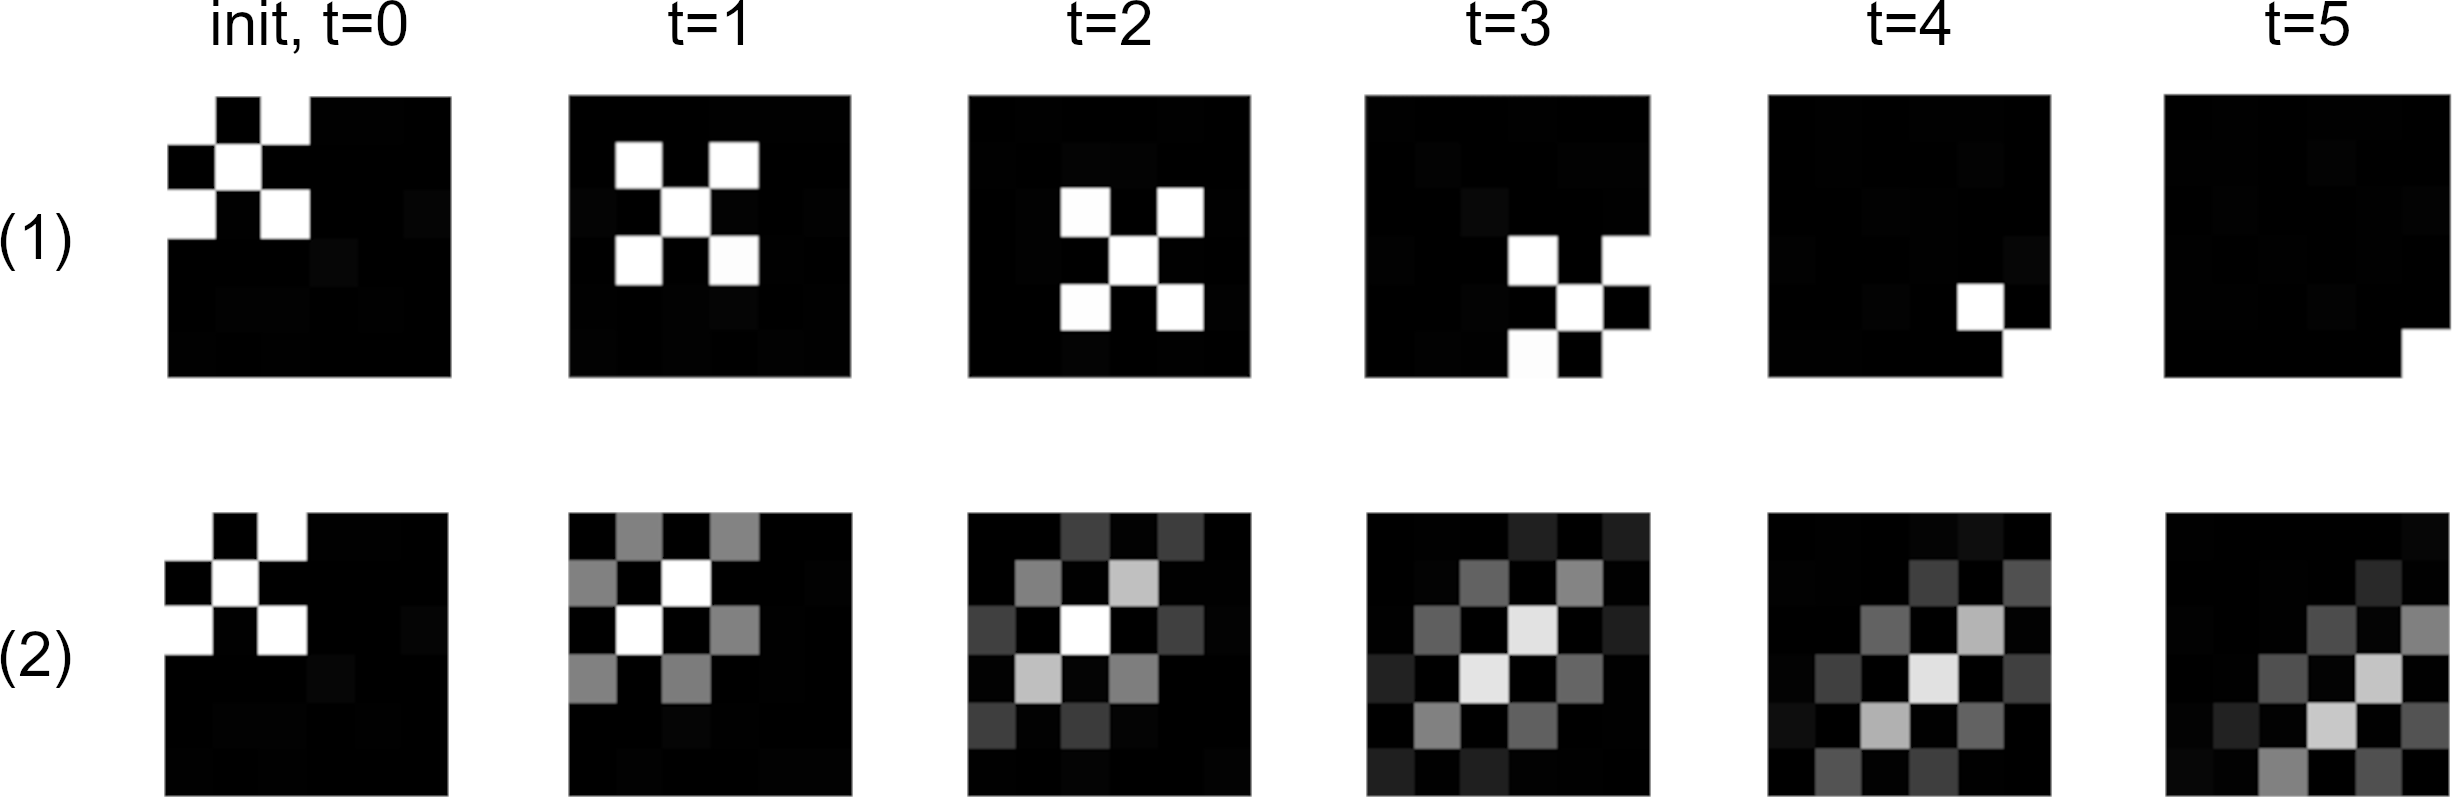
\includegraphics[width=0.9\linewidth]{Graphics/CA_examples.png}
    \caption{Examples of two elementary Cellular Automata on visual data. In a cellular automaton, the state of each cell (e.g., a pixel here) at time step $t+1$ is determined only by the states of the cell itself and its immediate neighbors at time step $t$. In this case, the 3x3 surrounding pixels. The update rules can be described as simple 3x3 kernels. Where time runs from left to right, and the filter is applied to each pixel in each time step. In example (1), there is only a simple shift, and in example (2), the original shape diverges and moves.}
    \label{fig:ca_exp}
\end{figure}

CAs are generally more complex than these simple examples and are not limited to visual data. Instead, among many other things, CAs can be used to simulate and model, e.g., urban evolution, turbulence phenomena, and other fundamental physics, and in general, many discrete dynamical systems, see, e.g., \autocite{Berto:StanfordSurvey_CA:2022}.

Thus, CAs exist for a long time and have a vast application potential. However, the main challenge in directly modeling CAs is often finding a suitable update rule \cite{Gilpin:2019:IntroduceNCA}. In Neural Cellular Automata, these update rules are modeled or trained with a neural network, which is discussed in more detail in the following section.
\section{Neural Cellular Automata}
\label{methods:NCA}
%%%% --- NCA allgemein --- %%%%
Finding an appropriate update rule is often a particular challenge when modeling CAs \cite{Gilpin:2019:IntroduceNCA}. In NCAs, this update rule is learned using a Neural Network (NN). A Neural Cellular Automaton (NCA) is, therefore, a simple (i.e., small) Neural Network. In image processing, the neighborhood of the CA is usually the pixel grid of the input image. Since the update rule is based only on the "direct" neighbors, the NN in an NCA is limited to using only tiny (e.g., 3x3) filter kernels. These architectural choices make the model very small regarding the number of parameters. In addition, unlike other NNs, NCAs do not pass the input through the model just once to generate the output. Instead, the output is fed back into the model for a fixed number of time steps ("inference steps"). In terms of a CA, we let the model update the state (neighborhood) for a fixed number of iterations until we observe the image state. Then, the loss is computed and backpropagated through the model as in any other NN. 

In addition, NCAs also use additional channels, i.e., a hidden state that is many times larger than the input. This hidden state and the input image form the hidden input and output of NCAs, which are used only by the model itself. This allows the model to spread information over the entire image, even if it takes several time steps. The intermediate states are overwritten at each step, i.e., they are not stored, and only a layer the size of the input image is used for the final output. The hidden state is not used for loss calculation.


%%%% --- Models --- %%%%
\label{methods:NCA:Models}
We used two different NCAs for training. The Backbone-NCA and the Med-NCA, as shown in \autoref{fig:NCA_Models}. The Med-NCA is built from two backbone NCAs. Both models are designed for medical image segmentation and were developed by \cite{kalkhof:2023:medNCA}. Although they can be used with different numbers of inference steps and channels, we have consistently used 64 inference steps and 16 channels, which are zero-seeded. Only 15 channels can be used by the model because the first channel is overwritten with the original input image after each inference step. The standard Med-NCA configuration uses 32 channels but provides only 0.01 more performance on Dice, while the 16-channel variant requires 2.5 times fewer parameters. The Backbone NCA is about 0.033 weaker on Dice than the Med NCA, although this also depends significantly on the training set \cite{kalkhof:2023:medNCA}.

Another difference between the NCAs we used and most other NNs is that they use randomness, e.g., during inference. In each inference step of the model, only a random portion of the computed output is returned to the model in the next inference step. That way, the model can continue to compute only a portion of the previous output in the next iteration. The output is randomly masked with $p=0.5$. This is similar to other NCA approaches in image processing \cite{mordvintsev:2020:growingNCA, sandler:2020:imageSegNCA}. The goal behind the randomness is to simulate asynchronous execution. Both models use kernels of size $3\times3$. Overall, tiny but robust models can be trained this way. 


%%%% --- Backbone-NCA --- %%%%
\subsection{Backbone-NCA}
The Backbone-NCA is build with a simple architecture, as can be seen in \autoref{fig:NCA_Models}. The Backbone NCA is only the one on the right. However, it is a powerful segmentation NCA. According to the ablation study by \cite{kalkhof:2023:medNCA}, it is only slightly weaker than the med-NCA on the hippocampus dataset we also used. Because of its simple architecture and good performance, we decided to explore using this NCA and this dataset first and then see if any results could be replicated on the Med-NCA and other datasets.

The backbone NCA consists of 2 conv2d layers, which are limited to a kernel size of $3\times3$ and have an input and output depth corresponding to the channels, i.e., 16 in our experiments. These two layers are arranged in parallel, and their output is merged with the input via two linear layers with intermediate Relu. This model block is run through in each inference step. After each inference step, the generated output is merged with the original input again, forming the input for the next inference step. After all (in our case 64) inference steps, the loss is computed using the ground truth labels and propagated back using the PyTorch \cite{paszke:2019:pytorch} backward function.


%%%% --- Med-NCA --- %%%%
\subsection{Med-NCA}  
\label{methods:NCA:Med-NCA}
The Med-NCA is the more powerful segmentation NCA we use. It is build of two Backbone-NCAs and uses additional up- and downscaling and patching, as can be seen in \autoref{fig:NCA_Models}. For this reason, we decided to test the transferability to another model with this NCA after the results could be achieved with the Backbone NCA. We also used it to test the transferability to the more difficult prostate dataset. 

It is based on 2 Backbone-NCAs connected in series. The first Backbone-NCA works with low-resolution inputs. After the 64 inference steps of the first NCA, the output is scaled up again and sent to the second NCA together with the input image. The second NCA continues to work directly on the output of the first NCA at a higher resolution. The second NCA trains on patches to reduce the VRAM. This is no longer necessary after training. The loss is only calculated on the final output and fed back through both models after the second model has also been executed with 64 inference steps.

\begin{figure}[h!]
    \centering
    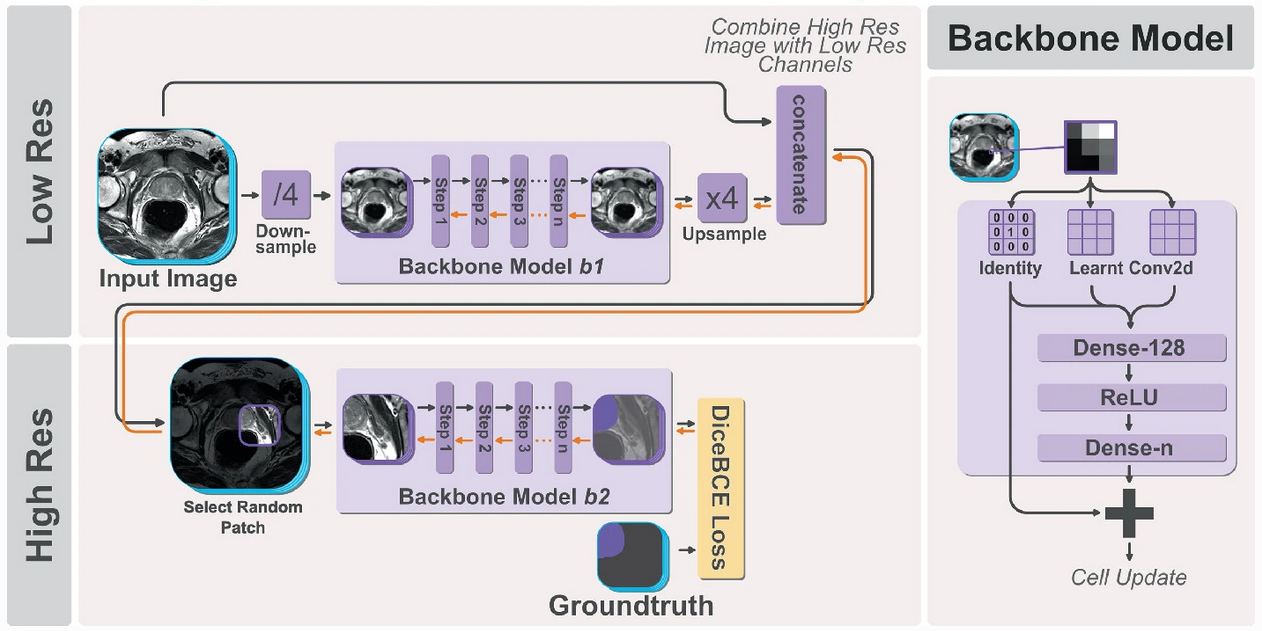
\includegraphics[width=\linewidth]{Graphics/MedNCA_2D.png}
    \caption{The NCAs we used. On the right: The Backbone-NCA, a simple architecture. Whole image: The Med-NCA, using 2 Backbone-NCAs. One training on the whole image, but with low resolution, and one training on high-resolution patches. Patching is not needed after training but reduces VRAM usage. When using the Backbone-NCA alone, we also used the DiceBCE loss. Models and image from \cite{kalkhof:2023:medNCA}.}
    \label{fig:NCA_Models}
\end{figure}

%%%% --- DiceBce Loss --- %%%%
\subsection{DiceBCE Loss}
\label{DiceBCE-Loss}
Both the Backbone-NCA and the Med-NCA use the DiceBCE as the loss. The DiceBCE consists of two parts: the complement of the S{\o}renson-Dice coefficient (Dice or Dice-Loss) and the Binary Cross Entropy (BCE). The DiceBCE is simply the addition of the Dice-Loss and the BCE (\ref{eq:DiceBCE_1}). We use 'Dice' inconsistently for both the complement (i.e. as loss) and the score itself, although it should be apparent from the context what is meant. In particular, only the complement is used as the loss, and only the S{\o}renson-Dice coefficient itself is used as the score for testing, and we never form the complement of the complement or anything like that.

The Dice is the harmonic mean of precision and recall (\ref{eq:DiceBCE_2}), which can be transformed to (\ref{eq:DiceBCE_3}), where TP, FP, and FN stand for True Positive, False Positive, and False Negative, respectively. Overall, the Dice also emphasizes true positives over false positives. For an image volume, where $x_n$ is a prediction $\in(0,1)$ and $y_n$ is a ground truth label $\in(0,1)$ and $n$ is the size of the vectors, i.e., the size of the image volume is $n$. The dice can then be rewritten as (\ref{eq:DiceBCE_4}), where a smoothing factor is added to avoid zero derivatives.

The BCE weights the prediction and rejection ($x_n$ and $(1-x_n)$) logarithmic before multiplying them by the ground truth and then adding them. This element weighting is done for operations on vectors, such as image volumes, where we then reduce by the mean (\ref{eq:DiceBCE_5}). The BCE also maximizes the logarithmic weighted correct predictions of the model and thus minimizes the logarithmic weighted incorrect predictions. The DiceBCE also maximizes the logarithmic weighted correct predictions of the model with a shift towards the true positives.

We used the binary cross entropy function from PyTorch \cite{paszke:2019:pytorch} with reduction for the BCE.
This version of the DiceBCE was used for both the Backbone-NCA and the Med-NCA and proved very effective. Therefore, we used it as a reference in our experiments, and as a starting point for other loss functions we tested.

\begin{align}
    \mathrm{DiceBCE}    &:= 1 - \mathrm{Dice} + \mathrm{BCE},           \label{eq:DiceBCE_1}\\[10pt]
    \mathrm{Dice}       &:= 2 \cdot \frac{\mathrm{precision} \cdot \mathrm{recall}}
                                            {\mathrm{precision} + \mathrm{recall}}          \label{eq:DiceBCE_2}\\[10pt]
                        &= \quad \frac{2 \cdot \mathrm{TP}}
                                   {2 \cdot \mathrm{TP} + \mathrm{FP} + \mathrm{FN}}        \label{eq:DiceBCE_3}\\[10pt]
                        &= \quad \frac{2 \cdot {\sum(x_n \cdot y_n)} +1}
                                   {\sum(x_n) + \sum(y_n) +1}                               \label{eq:DiceBCE_4}\\[10pt]
   \mathrm{BCE}         &:= \mathrm{mean}\ ( -[y_n \cdot \log x_n + (1-y_n) \cdot \log (1-x_n)])        \label{eq:DiceBCE_5}
\end{align}
%%%% NQM %%%%
\section{NCA Quality Metric (NQM)}
\label{methods:NQM}
\begin{figure}
    \centering
    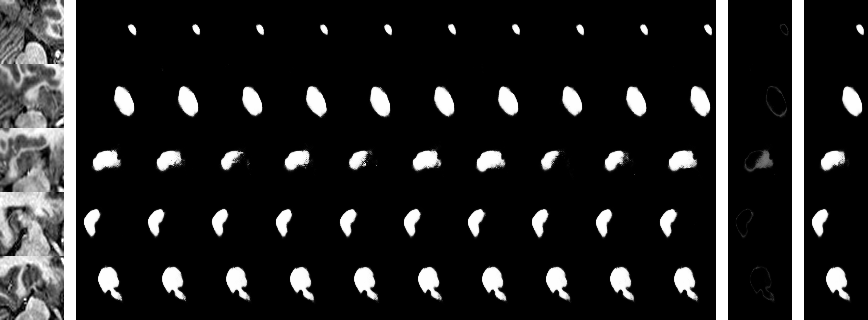
\includegraphics[width=\linewidth]{Graphics/nqm_stack10_epoch_50_var_mu.png}%{Graphics/nca_random_outputs.png}
    \caption{From left to right: Inputs, 10 predictions, Variance, and Mean. As seen here, NCAs produce different outputs on identical inputs each time they are called. Each of the 10 predictions here are outputs of the same model. Therefore, as shown on the right, one can compute a variance and a mean over these predictions. The NQM we introduce here for model optimization reduces this to single values. The outputs are generated from a model in an earlier training state for better visualization.}
    \label{fig:nca_random_outputs}
\end{figure}

%%%% random activation + image example %%%%
As seen in \autoref{methods:NCA}, NCAs are activated randomly to a certain extent. Therefore, they generate different predictions each time they are called, especially with the same input. Examples can be seen in \autoref{fig:nca_random_outputs}. On the far left, one can see five different inputs. Next to them are ten outputs from the same model, shown here for better visualization at an early stage of training. Especially for the middle input, the differences in the outputs can be seen quite well with the naked eye. For the other inputs, the variance over these ten outputs (the second last column on the right) also clearly shows that the model produces different outputs for all input images. Otherwise, the variance should be zero, i.e., completely black. The variance decreases for models with higher epochs but never disappears. It also remains the case that the variance for some inputs is significantly worse than for others.

%%%% Def NQM, from/like John %%%%
\autocite{kalkhof:2023:M3D-NCA} introduced a way to measure this stochasticity of NCAs, caused by random activation, by computing a mean-normalized variance over a stack of such generated outputs and named it the NCA-\textit{Quality-Metric} (NQM). \autocite{kalkhof:2023:M3D-NCA} used this to detect bad segmentation on artificially degenerated data automatically. They defined it as follows, with $v$ as the image volume and $v_i$ as $N=10$ different predictions:

\begin{align}
    \mathrm{NQM} := \frac{\sum_{s\in SD} (s)}  {\sum_{m\in\mu}}, \qquad
    \mathrm{SD} = \sqrt{\frac{\sum^N_{i=1}(v_i-\mu)^2}  {N}}, \qquad
    \mu = \frac{\sum^N_{i=1}v_i}  {N}
\end{align}


This approach has given rise to the question of whether it is possible somehow to pull the NQM inside the training circle, to improve the robustness of the models and not just for the final evaluation. What has been addressed with this thesis. 


%%%% Why to put NQM in the Loss %%%%
The NQM is a single scalar value greater than or equal to zero. With the NQM, a model will perform better if the NQM is smaller. Therefore, the goal of optimizing a model with respect to the NQM can be formalized as a direct minimization problem over the NQM $\min(\text{NQM})$. Other approaches are possible, as discussed in \autoref{conclusions}. Since the object to optimize the NQM can be formalized as a minimization problem, and in the training cycle of a Neural Network, there is already an object to minimize, i.e., the loss, and NCAs are Neural Networks, it is very close to trying to minimize the NQM by using it as the loss function or by including the NQM in the loss function. This is also our approach in this work, and, as we will show, it can lead to a more robust behavior of the model. I.e., it can improve the robustness of the model, as we will see in \autoref{experiments:intro} especially in \autoref{experiments:03.1.0:backbone_hippo:intro}. In \autoref{experiments:03.2.0:med_prost:intro}, \ref{experiments:03.3.0:med_hippo:intro_and_Augmented}, and \ref{experiments:03.4.0:backbone_prost:intro}, we will also see that this is not trivial to transfer to other models and datasets, and that some models may even become less robust.


%%%% Schlussanmerkung  -> evt. nach Conclusions %%%%
The NQM, and therefore this approach, is limited to NCAs and possibly other models with randomness in the output since it is a metric over that randomness. Therefore, the NQM and everything related to it in this paper does not work for most other Neural Networks since the output with these is deterministic.
    \chapter{Experiments}
\label{experiments:intro}

%%%%% Overview %%%%%%
In this chapter, we focus on the experiments we conducted to investigate whether and to what extent the NQM (\autoref{methods:NQM}) can be used to increase the robustness of NCAs. \autoref{Experiments:OverviewTree} gives a condensed overview for the experiments. The experiments can be divided into three blocks: First, the tests whether the NQM can be implied as a loss at all (\autoref{experiments:01.0:Into}), secondly, the construction of functioning losses (\autoref{experiments:02.0:intro}), and thirdly, the robustness tests and improvements (\autoref{experiments:03.0:Intro}). These three build on each other logically and were executed in this order. However, this is only partially the case within the sections. More often, several strands were explored simultaneously, and there are some cross-connections. These sections are organized thematically and do not build on each other chronologically or logically.\\
In \autoref{experiments:01.0:Into}, we first investigated whether the NQM could be implemented directly as a loss. This was preceded by a detailed evaluation of the existing setup, which also considered other ways of making the NQM usable. For example, by duplicating the samples for which the NQM is particularly poor in an interim evaluation. This could be done once or several times in the training cycle after a fairly large number of epochs. See also Future Works (\autoref{future_work}). However, the implementation as a loss was initially seen as the most promising solution. In \autoref{experiments:01.0:Into} we will only consider that this is technically possible in principle.\\
Subsequently, in \autoref{experiments:02.0:intro}, the goal was to develop a loss that is either better than the standard loss of the existing training setup or at least no worse. Ultimately, the latter was the case.
Finally, in \autoref{experiments:03.0:Intro} we were able to apply this loss function developed in \autoref{experiments:02.0:intro} in a simple setup on different perturbed datasets to increase robustness (\autoref{experiments:03.1.1:backbone_hippo:spike_noise}).\\
We then applied this to a more sophisticated model and dataset. However, there were fewer positive results here (\autoref{experiments:03.2.0:med_prost:intro}), so we decided to investigate the transferability further. For this purpose, we conducted experiments separately for model and dataset to narrow down the problem area (\autoref{experiments:03.3.0:med_hippo:intro_and_Augmented} and \autoref{experiments:03.4.0:backbone_prost:intro}). The results here indicate that with the approach chosen here, it is primarily the dataset that is challenging in terms of transferability and less so the model.
Furthermore, we simultaneously conducted additional tests with the successful setup (\autoref{experiments:03.1.2:backbone_hippo:pretrained}) and investigated hyperparameters (\autoref{experiments:03.1.w:Hyperpatameters}) and further loose (\autoref{experiments:03.1.x:FurtherNQMLosses}).

%%%%% Overview - Tree %%%%%%
\begin{figure}[h!]
    \centering
    \tikzstyle{selected}=[draw=red,fill=red!30]
    \tikzstyle{done}=[fill=green!45]
    \tikzstyle{tables done}=[fill=yellow!45]
    \tikzstyle{optional}=[dashed,fill=gray!50]
    \begin{tikzpicture}[dirtree]
    \node [selected] {\ref{experiments:01.0:Into} experiments}
        child { node {\ref{experiments:01.1:Only_NQM} Only NQM}}	
        child { node {\ref{experiments:02.0:intro} Dice, Bce and NQM}
            child { node {\ref{experiments:02.1:diceBce+NQM} DiceBceNQM}}
            child { node {\ref{experiments:02.2:FurtherDice-Bce-NQMLosses} Further Mixed Dice-Bce-NQM Losses}
                % child { node {\ref{experiments:02.2.1:Only_NQM_Pretrained} On Pretrained Models}}
                % child { node {\ref{experiments:02.2.2:dice+NQM} Multiplicative Dice-Bce-NQM Losses}}
            }
        }
        child { node {\ref{experiments:03.0:Intro} Robustness Improving}
            child { node {\ref{experiments:03.1.0:backbone_hippo:intro} Backbone-NCA on Hippocampus}
                child { node {\ref{experiments:03.1.1:backbone_hippo:spike_noise} Augmented Datasets}}
                child { node {\ref{experiments:03.1.2:backbone_hippo:pretrained} Pretrained Models}}
                child { node {\ref{experiments:03.1.w:Hyperpatameters} Hyperparameters}
                    child { node {\ref{experiments:03.1.3:backbone_hippo:stackSize} stacksize 2, 3, 6}}
                    child { node {\ref{experiments:03.1.4:backbone_hippo:alpha} alpha 0.5 and 2.0}}
                }
                child { node {\ref{experiments:03.1.x:FurtherNQMLosses} Non-Linear NQM Losses}
                    child { node {\ref{experiments:03.1.5:backbone_hippo:logNQM} logNQM bases 2, e, 3, 10}}
                    child { node {\ref{experiments:03.1.6:backbone_hippo:powNQM} powNQM base 3}}
                    child { node {\ref{experiments:03.1.7:backbone_hippo:sqrtNQM} sqrtNQM}}
                }
            }
            child { node {\ref{experiments:03.2.0:med_prost:intro} Med-NCA on Prostate}
                child { node {\ref{experiments:03.2.1:med_prost:augmented} Augmented Datasets}}
                child { node {\ref{experiments:03.2.2:med_prost:onDomainShifts} Domain Shifts}}
            }
            child { node {\ref{experiments:03.3.0:med_hippo:intro_and_Augmented} Med-NCA on Hippocampus}}
            child { node {\ref{experiments:03.4.0:backbone_prost:intro} Backbone-NCA on Prostate}
                child { node {\ref{experiments:03.4.1:backbone_prost:Augmented} Augmented Datasets}}
                child { node {\ref{experiments:03.4.2:Backbone_prost:DomainShifts} Domain Shifts}}
            }
        };
    \end{tikzpicture}
    \caption{Condensed overview of our experiments}
    \label{Experiments:OverviewTree}
\end{figure}

%%%%% Datasets %%%%%
\subsection*{Datasets}
\begin{figure}[h]
    \centering
        \begin{minipage}{0.49\textwidth}
        \centering
        %\includegraphics[width=0.9\textwidth]{example-image-a} % first figure itself
        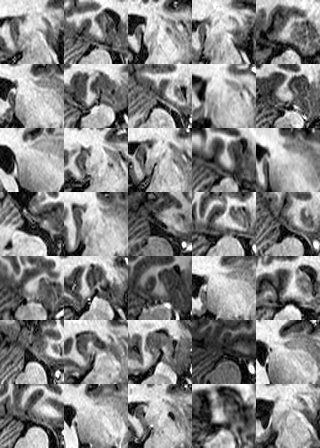
\includegraphics[width=\linewidth]{Graphics/datasets/dataset_hippo_examples_small.png}
    \end{minipage} \hfill
    \begin{minipage}{0.49\textwidth}
        \centering
        %\includegraphics[width=0.9\textwidth]{example-image-b} % second figure itself
        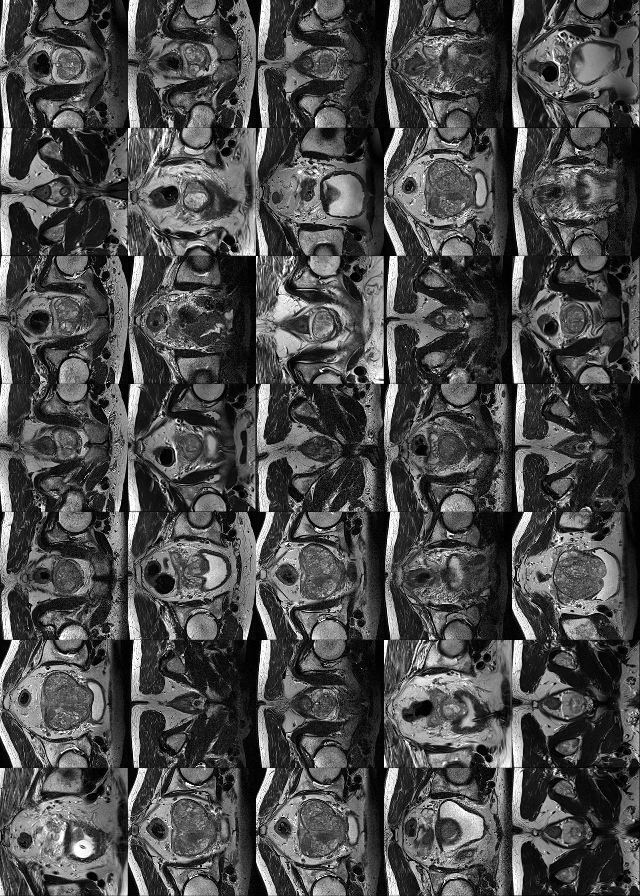
\includegraphics[width=\linewidth]{Graphics/datasets/dataset_prost_examples_small_highRes.png}
    \end{minipage}
    \caption{Example volumes from the main datasets we used. The hippocampus (left) and the prostate (right)}
    \label{fig:datasets:prost_hippo_examples}
\end{figure}

Initially, we trained mainly with the hippocampus dataset from \cite{Antonelli:2022:MedSegmentationDecatlon} and later included the prostate dataset to test transferability. The hippocampus dataset contains 394 3D volumes, and the prostate dataset has 48. We always used the train-test split of 0.7 to 0.3, indexed by \cite{Antonelli:2022:MedSegmentationDecatlon}. Some of these labels are not public. We have filtered them out. Therefor, we have 260 vital hippocampus and 26 vital prostate 3D volumes. Since these are 3D datasets, but the models we used work with 2D data, we sliced each volume. Thus, we obtained 6505 training and 2765 test 2D volumes with the hippocampus dataset and 352 training and 133 test 2D volumes with the prostate dataset. Examples can be found in \autoref{fig:datasets:prost_hippo_examples}.

\subsection*{Robustness}
\label{methods:Robust}

%%%% allgemein %%%%
In order to make robustness statements about our models (\autoref{experiments:03.0:Intro}), we generated static datasets and evaluated them continuously on the dice score. We mainly used the hippocampus and prostate datasets from the Medical Segmentation Decathlon \cite{Antonelli:2022:MedSegmentationDecatlon}. 

%%%% Augementation %%%%
We used both augmented datasets to test robustness against artifacts when they were not included in the training set and against artifacts when they were included in the training set. For the augmentations, we used the RandomSpike function and a slightly modified version of the RandomNoise function from the 'Augmentation' package of the torchIO Python library \cite{torchIO}.

%%%% DomainShifts %%%%
To test against domain shifts, we used data from 4 prostate datasets from the  
Medical Segmentation Decathlon \cite{Antonelli:2022:MedSegmentationDecatlon} (decathlon), 
parts of the UCL prostate dataset \cite{Ahmed:2017:UCL_PROMIS},
IEEE International Symposium on Biomedical Imaging \cite{Bloch:2015:ISBI_Data, Clark:2013:ISBI_TCIA} (ISBI), and the
Initiative for Collaborative Computer Vision Benchmarking \cite{Lematre:2015:i2cvb} (i2vb). We then used these to generate several domain-shifted datasets artificially. To do this, we inserted single or multiple datasets from one dataset into another, trained on them, and evaluated them on the original datasets. In addition, we generated a dataset from all prostate data available to us, trained models with different losses on it, and evaluated them on the original and training datasets.


%%%%% System %%%%%
\subsection*{System}
\label{experiments:intro:system}
We mainly trained on a system with a single NVIDIA GeForce RTX 4090, 16 AMD Ryzen 7 5700G with Radeon graphics and 58.7 GiB of main memory. The RTX 4090 has 24 GiB of VRAM, which we mostly used completely. This system was used for most tests, especially all quantitative statements and comparisons.\
Some qualitative statements are based on tests run on a other system, with seven Tesla T4, 40 Intel Xeon Silver 4210 CPU with 2.20GHz and 260GiB main memory. But there we always used only a single gpu and a single cpu. A Tesla T4 got around 16 GiB of VRAM. 


%%% --- inputs ---
\section{NQM as Lossfunction}
\label{experiments:01.0:Into}

We decided to investigate whether it is possible to include the NQM in the training loop to improve the robustness of the model by implementing the NQM directly as a loss function  or using it inside of it. To make sure that this is even possible, but also as a sensible first step in this direction, we decided to implement the NQM directly as a loss function.

In this section, we will see our first attempts to do so as a proof of concept but also to illustrate the problems that arise when using only the NQM as a loss. First, we will see in \autoref{experiments:01.1:Only_NQM} that it is technically possible to use the NQM directly as a loss function but that it has no use for training. This is because the NQM itself does not consider the label; therefore, the model will always take the opportunity to minimize the NQM as a loss by fitting into an all-one label.

%%% input %%%
%\subsection{Only NQM as a Loss}
\label{experiments:01.1:Only_NQM}
Therefore, as a first attempt at the use of the NQM for robustness, we simply defined the NQM itself as a loss:

\begin{align}
    \mathrm{NQM}\ :=\ \frac{\sum_{s\in SD} (s)} {\sum_{m\in\mu}}, \qquad
    SD = \sqrt{\frac{\sum^N_{i=1}(v_i-\mu)^2}  {N}}, \qquad
    \mu = \frac{\sum^N_{i=1}v_i}  {N}  
\end{align}

However, using this as a loss function does not work because the values below the square root in the SD and the denominator of the NQM can become zero and are then undefined.
To avoid zero-squarerooting, we choose to add an $\varepsilon$ of $e^{-8}$. To avoid zero-division, we choose to add a smoothing value of $1$. This makes the NQM loss:

\begin{align}
    \mathrm{NQM}\ :=\ \frac{\sum_{s\in SD} (s) {\color{red}+1}} {\sum_{m\in\mu} {\color{red}+1}}, \qquad
    SD = \sqrt{\frac{\sum^N_{i=1}(v_i-\mu)^2}  {N} {\color{red} + \varepsilon}}, \qquad
    \mu = \frac{\sum^N_{i=1}v_i}  {N}  
\end{align}


Loss function technically works. The model can be trained on it, but it will simply label the entire image within very few epochs since the NQM will be zero if the denominator becomes as large as possible, which is the case if the prediction is maximized. So, a model trained on this loss function will not predict anything because it will predict everything.\\
The loss function is usually a function of a model output and a label $\ell(y_i, f_\theta(x_i))$. However, since the NQM is only a function of the model output $\ell(f_\theta(x_i))$, it is not possible that a model trained on the NQM can predict anything. Therefore, it is a crude but sensible first step in exploration.


\begin{figure}[h!]
    \centering
    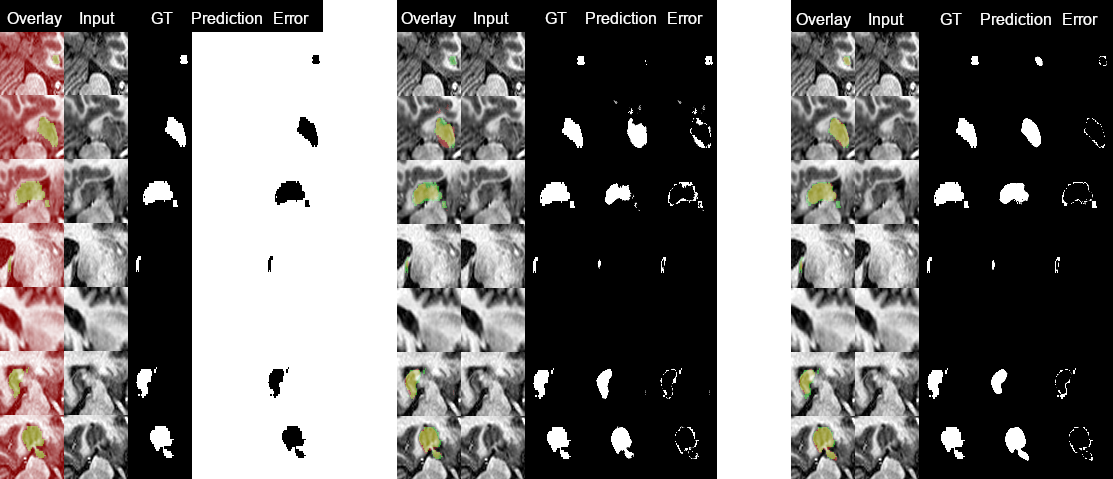
\includegraphics[width=\linewidth]{Graphics/Experiments/4.1.1_DiceBce_GT_vs._NQM_only_v2.png}
    \caption{Example image volumes (input) with ground truth labels (GT), predictions and errors. The overlay shows the input image with false positive (red), true positive (yellow), false negative (green). The model on the left was trained on the NQM as loss and clearly predicts nothing at all by simply labeling everything (overlay all red, label all white). The output stays this way from epoch 2 on. For comparison, the middle and right models were trained on DiceBCE. The middle one shows the output after 10 epochs, the right one after 500 epochs.}
    \label{fig:exp.01.1:DiceBce_vs_NQM_only}
\end{figure}           % section
\section{Dice, Bce and NQM}
\label{experiments:02.0:intro}
We decided to investigate whether it is possible to include the NQM in the training loop to improve the robustness of the model by implementing the NQM directly as a loss function or using it within the training loop. However, as seen in \autoref{experiments:01.0:Into}, it is technically possible but not very useful to use the NQM as a loss on its own. Therefore, in this section, we will focus on our attempts to implement a loss function that takes the NQM into account but not depends only on it. In \autoref{experiments:02.1:diceBce+NQM}, we will see the implementation that has worked best here, and which we have also used for most of the robustness improvement experiments (\autoref{experiments:03.0:Intro}). For completeness, the rest of this section will show some other attempts at loss functions that worked worse or not at all and that we discarded after testing them here. We also tested some other implementations not presented here, particularly those we re-tested in \autoref{experiments:03.1.x:FurtherNQMLosses}. These did not show any improvement over the DiceBceNQM loss here. They will be presented in \autoref{experiments:03.1.0:backbone_hippo:intro} for compactness.


The goal for the experiments in this section was to implement the NQM in the loss function so that the quality of the model improves or at least does not degrade. So we can build on this for robustness improvement. Therefore, we are working on the original dataset, and we used the Backbone-NCA and the Medical Segmentation Decathlon Hippocampus dataset \cite{Antonelli:2022:MedSegmentationDecatlon} and the Backbone-NCA default loss function, the DiceBCE, for comparison.


%%% --- inputs ---
\subsection{Additive Dice-Bce-NQM Loss}
\label{experiments:02.1:diceBce+NQM}
\begin{figure}[h!]
    \vspace{0.5cm}
    \centering
        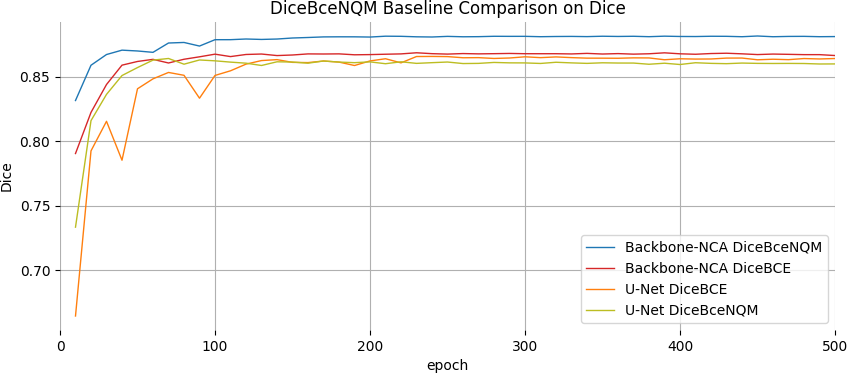
\includegraphics[width=\linewidth]{Graphics/Experiments/2.1_inverted_freeAxes_Loss_DiceLoss()_test_mask0.png}
        \caption{Backbone-NCA trained on DiceBceNQM (blue). For comparison, as baselines, a Backbone-NCA trained on DiceBCE and two U-Nets are given. The convergence of the Backbone-NCA on DiceBceNQM is quite similar to the Baselines. Therefore, training is stable on this loss regarding the Dice score. The U-Nets have been trained for 1000 epochs in total, but the Dice does not change any further, even so the train loss does.}
    \label{fig:02.1:DiceBceNQM:Baselines:onDice}
\end{figure}

As we have seen in \autoref{experiments:01.0:Into}, using only the NQM as a loss function cannot work because the reference to the ground truth label is missing, and since the models we use, the Backbone-NCA as well as the Med-NCA, already use a well working loss; the DiceBCE given in \ref{DiceBCE-Loss} is close to it, to go from there. In this way, we have developed a working NQM-loss function, which works as well as the DiceBce in our first tests, just by adding the NQM to the DiceBCE. The DiceBceNQM, as we later used it mainly for our robustness improvement experiments.

Since the NQM can be very large in the initial training cycles, we additionally cropped the NQM to a value of $\in(0,1)$ to relax the weight of the NQM in the total loss. This results in the DiceBceNQM as follows:

\begin{align}
    \text{DiceBceNQM} &:= 1 - \mathrm{Dice} + \mathrm{Bce} {\color{red}+} \mathrm{NQM},\label{eq:02.1:DiceBceNQM}\\           
    \mathrm{NQM}\ &:=\ \min\left(1, \quad \frac{\sum_{s\in SD} (s) +1} {\sum_{m\in\mu} +1}\right), \qquad
    SD = \sqrt{\frac{\sum^N_{i=1}(v_i-\mu)^2}  {N}  \varepsilon}, \qquad
    \mu = \frac{\sum^N_{i=1}v_i}  {N}               \label{eq:02.1:Only_NQM}
\end{align}

As can be seen in \autoref{fig:02.1:DiceBceNQM:Baselines:onDice} (for Dice), \autoref{fig:02.1:DiceBceNQM:Baselines:onTrainLoss} (for train losses), the Backbone-NCA converges on the DiceBceNQM about as well as on the DiceBCE, measured on Dice, or even slightly better (+1.8 points). We also trained two U-Nets, one on the DiceBCE, the other on the DiceBceNQM, as additional baselines. The convergence is approximately similar to the Backbone-NCA trained on DiceBCE. Furthermore \autoref{fig:02.1:DiceBceNQM:Baselines:Segmentations} show segmentations for the final model and baselines. As can be seen by eye the predictions with the DiceBceNQM are as good as with the DiceBCE. Putting all this together, training on this loss is stable and reliable and as least as good as on the DiceBCE alone. Therefor we used it for most of our robustness tests in \autoref{experiments:03.0:Intro}. 

\begin{figure}[h!]
    \vspace{0.5cm}
    \centering
        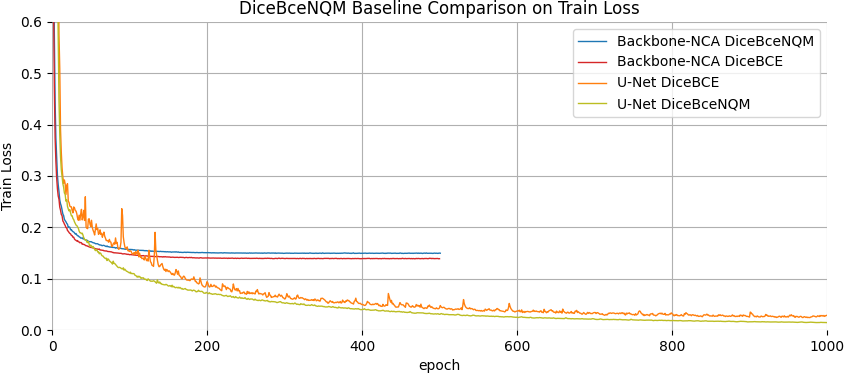
\includegraphics[width=\linewidth]{Graphics/Experiments/2.1_train_loss_freeAxes_Loss_train_0.png}
        \caption{Backbone-NCA trained on DiceBceNQM (blue). For comparison, as baselines, a Backbone-NCA trained on DiceBCE and two U-Nets are given. The convergence of the Backbone-NCA on DiceBceNQM is quite similar to the Baselines. Therefore, training is stable on this loss regarding. The U-Nets have been trained for 1000 epochs in total, Backbone-NCAs only 500 epochs.}
    \label{fig:02.1:DiceBceNQM:Baselines:onTrainLoss}
\end{figure}

\begin{figure}[h!]
    \vspace{0.5cm}
    \centering
        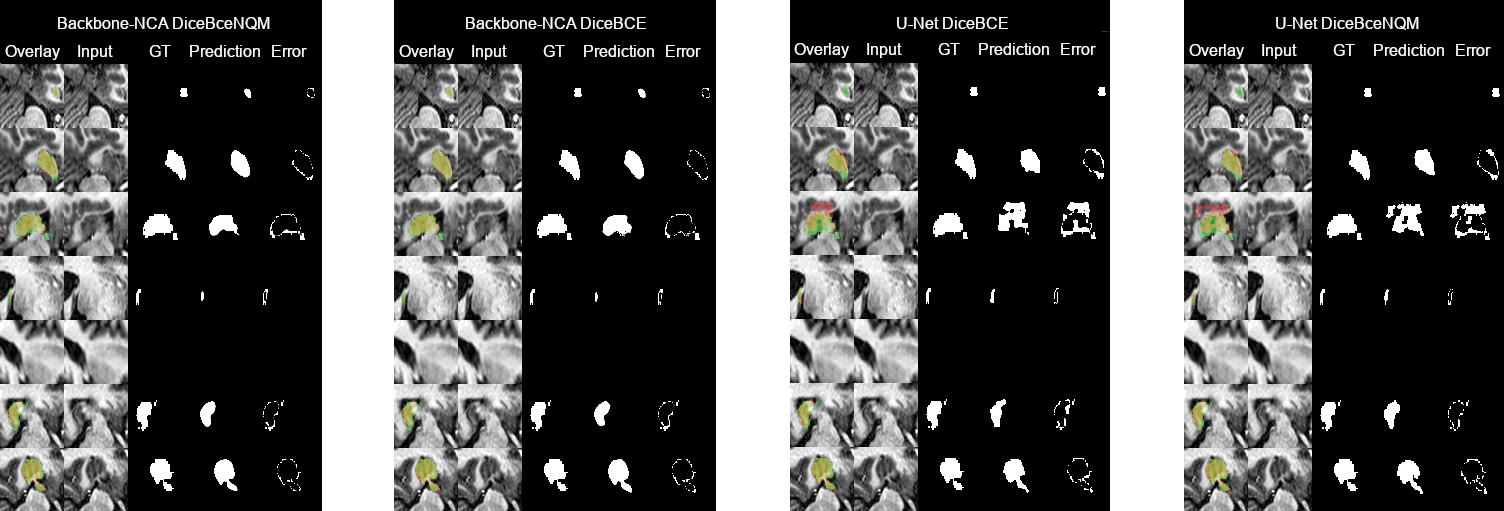
\includegraphics[width=\linewidth]{Graphics/Experiments/2.1_BaselineComparison.png}
        \caption{Backbone-NCA trained on DiceBceNQM (left). For comparison, as baselines, a Backbone-NCA trained on DiceBCE and two U-Nets are given. For each model the same image volumes (inputs) are given. With ground truth labels (GT), predictions, and errors. The overlay shows the input image with false positive (red), true positive (yellow), and  false negative (green). All for the final models after 500 epochs for Backbone-NCAs and 1000 epochs for U-Nets. First and foremost the predictions with the DiceBceNQM for the Backbone-NCA are at least as good as with the DiceBCE. Therefor training on the DiceBceNQM is stable. Even so some segmentations by the U-Nets look worse, then by the Backbone-NCAs, the Dice is is quite similar (\autoref{fig:02.1:DiceBceNQM:Baselines:onDice}).}
    \label{fig:02.1:DiceBceNQM:Baselines:Segmentations}
\end{figure}


We also tested different stacksizes and alpha-values, like in \autoref{experiments:03.1.0:backbone_hippo:intro} and here even in more configurations then there, but since, they did not show any effect here (but there), they are introduced in \autoref{experiments:03.1.0:backbone_hippo:intro}.                 % subsection
\subsection{Further Mixed Dice-Bce-NQM Losses}
\label{experiments:02.2:FurtherDice-Bce-NQMLosses}
%%%% Intro %%%% 
After and before we had our first successes with the DiceBceNQM loss (\autoref{experiments:02.1:diceBce+NQM}), in the sense that we were able to develop a loss that was no worse than the DiceBCE alone, we tried several other implementations to incorporate the NQM into the DiceBCE loss. However, they were all worse than the DiceBceNQM, or at least no better. However, since the DiceBceNQM was the simplest of the equally good losses, we decided, in the spirit of Occam's razor, to start the robustness experiments (\autoref{experiments:03.0:Intro}) with the DiceBceNQM. The more promising of these were tested again in \autoref{experiments:03.1.x:FurtherNQMLosses}, but showed no improvement over the DiceBceNQM in the experiments here without robustness testing, and were judged here to be more computationally expensive or were developed later and are therefore not yet available. These losses are presented in \autoref{experiments:03.1.x:FurtherNQMLosses} and are omitted here to avoid duplication, even though they are clearly better. For the sake of completeness, we list here the loss functions that are worth mentioning, even if they did not make it to the next round.

For the case of the additive DiceBceNQM (\autoref{experiments:02.1:diceBce+NQM}), we also tested whether taking only Dice+NQM or only Bce+NQM had a positive effect, but as suspected, this was not the case.


%%%% Offen / TODO %%%%
\iffalse
... hier stimmte irgendwas nicht ...
... diceBceMasks (Bce with no reduction) was used and the nqm was put in as weight, before the mean was build ... therefore the nqm was calculated pixelwise ... but did not work
\begin{align}
    \mathrm{DiceBceMaskNQM}     &= \mathrm{DiceLoss} + \mathrm{mean} (NQM_mask \cdot \mathrm{BCE})\\
    \mathrm{BCE}(x,y)           &=  -[y_n \cdot \log x_n + (1-y_n) \cdot \log (1-x_n)]\\
    \mathrm{DiceLoss}           &= 1 - \frac{2 \cdot {\sum^D(y \cdot f_\theta(x))}}
                                            {\sum^D(f_\theta(x)) + \sum^D(f_\theta(x))}
\end{align}
... diceBce SD
... Bce weighted with NQM


\fi
%%%% Inputs %%%%
\input{content/experiments/02_Dice_Bce_and_NQM/02.2.1_NQMLossOnPretrained}
\input{content/experiments/02_Dice_Bce_and_NQM/02.2.2_DiceBce_mul_NQM} % subsection                   % section
\section{Robustness Improving}
\label{experiments:03.0:Intro}
\begin{figure}[h!]
    \centering
    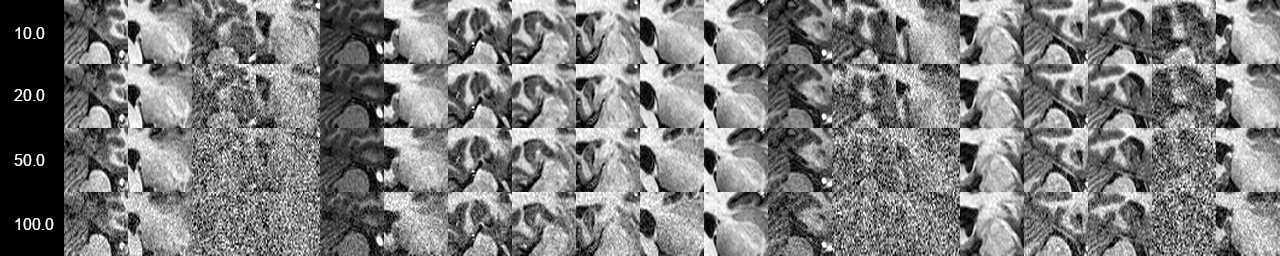
\includegraphics[width=\linewidth]{Graphics/datasets/datasets_hippo_randNoise_v2.png}\\
    \vspace{5pt}
    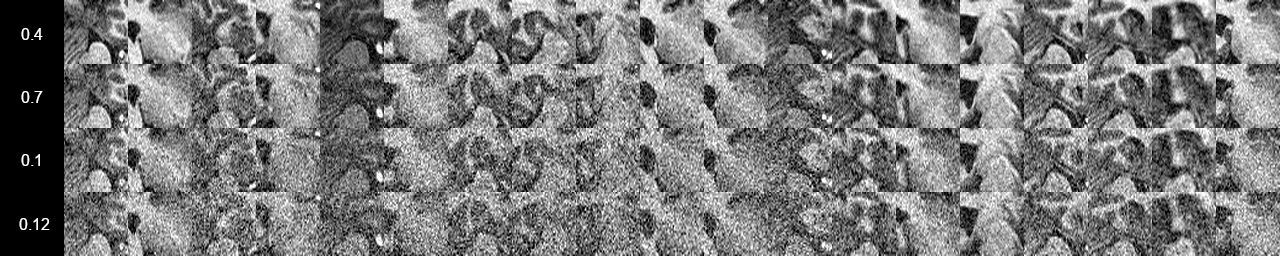
\includegraphics[width=\linewidth]{Graphics/datasets/datasets_hippo_normNoise_v2.png}
    \caption{Different noise functions that we tried for augmentation on the hippocampus dataset \cite{Antonelli:2022:MedSegmentationDecatlon}. The Standard deviation of the Gaussian distribution from which the noise is sampled is given on the very left. Top 4: Random noise function from torchIO \cite{torchIO}. As can be seen, the same images are always strongly affected. Bottom 4: Our simple addition to the random noise function with additional max-normalization, which we used for our test runs. As can be seen, the noise is much more evenly distributed across different images. Bottom 4: From top to bottom with increasing standard deviation in the noise function.}
    \label{fig:augemented:datasets:noise_problem}
\end{figure}

%%%% Allgemein Intro %%%%
Since in \autoref{experiments:01.1:Only_NQM} some adaptations of the DiceBCE loss with the NQM, all in front of the DiceBceNQM (\autoref{eq:02.1:DiceBceNQM}), no performance degradation could be seen, but also no improvement over the original data, we performed corresponding dedicated robustness tests. These are presented in this section.

Since \cite{kalkhof:2023:M3D-NCA} has already used the NQM to test the performance of models on augmented datasets in order to make robustness statements about the models, it is close to test, whether the DiceBceNQM improves robustness on a model, trained on perturbed data. To do this, we artificially perturb datasets. On the one hand with artificial augmentations to simulate different types of radiological image noise, on the other hand by adding individual data volumes from other datasets to our primary dataset to simulate data shifts.\\
As datasets, we mainly used the hippocampus and prostate datasets from the Medical Segmentation Decathlon \cite{Antonelli:2022:MedSegmentationDecatlon}. For the data shift, others accordingly (see below).

%%%% Augmentation %%%% 
For the augmentations, we statically generated four series of 5 perturbed datasets and the original dataset so that all models are trained on the same data. We used the hippocampus and prostate datasets from \autocite{Antonelli:2022:MedSegmentationDecatlon}. The datasets we generated are composed as follows and were selected according to the following criteria \begin{itemize}
    \item A series of 5 augmented datasets, each for the hippocampus and the prostate dataset, enriched with different proportions of spike artifacts.
    In each case, the goal was to decrease the dice performance of our GT model by 30 percentage points when all data were augmented ("Spike 1.0"). The four other datasets were then spiked with the same intensity, but only 0.3, 0.2, 0.1, and 0.01 shares of the data. We used the random spike function from the TorchIO package \autocite{torchIO}.
    We refer to these datasets as "Spike 1.0", "Spike 0.3", "Spike 0.2", "Spike 0.1", and "Spike 0.01", respectively. 
    \item A series of 5 augmented datasets, each on the hippocampus and the prostate dataset, using the same procedure but with random noise. We used an adapted variant of the random noise function from the TorchIO package \autocite{torchIO}. We have extended it with a simple max-normalization so that the noise is distributed much more homogeneously across the different images of the dataset, and the noise function can still be used together with the other functions of the package. The difference can be seen in \autoref{fig:augmented:datasets:noise_problem}. The problem was that in the hippocampus dataset, the max-value for the volumes varies a lot, and the standard noise function does not normalize for this.
    We refer to these datasets as "Noise 1.0", "Noise 0.3", "Noise 0.2", "Noise 0.1", and "Noise 0.01", respectively.
\end{itemize}

%%%% DomainShifts %%%%
For the domain shifts, we used data from 4 prostate datasets from the  
Medical Segmentation Decathlon \cite{Antonelli:2022:MedSegmentationDecatlon} (decathlon, decath), which we used as the main dataset. We inserted parts of other datasets into this dataset. Namely, parts of the prostate dataset from the PROMIS study \cite{Ahmed:2017:UCL_PROMIS} (ucl), the
IEEE International Symposium on Biomedical Imaging prostate dataset \cite{Bloch:2015:ISBI_Data, Clark:2013:ISBI_TCIA} (isbi), and the
Initiative for Collaborative Computer Vision Benchmarking Prostate dataset \cite{Lematre:2015:i2cvb} (i2vb). Here, we have generated a total of 2 series of datasets:\begin{itemize}
    \item A series of the decathlon dataset and 3 "shift" datasets, where we have added a sample from another dataset to the decathlon dataset. We call these "decath," "shift 1 isbi," "shift 1 i2cvb," and "shift 1 ucl," respectively.
    \item A series of the decathlon dataset and 3 "shift" datasets, where we added several samples from another dataset to the decathlon dataset because no or little change was seen in the shift 1 datasets. In each case, we aimed for a drop of about 15 points on the dice score. This dropped at very different rates, so we added four samples for ucl (dice drop 13.6), eight samples for i2cb (dice drop 15.8), and 12 samples for isbi (dice drop 16.7).
    We call this "decath," "shift 12 isbi," "shift 8 i2cvb," and "shift 4 ucl," respectively.
    \item As well as one dataset from all our available samples. We call this "all joined".
\end{itemize}

%%%% Beides %%%%
To get as broad a picture as possible, we trained at least one series for each variation of our loss functions that we tested, both for the augmentations and domain shifts. For each series that we tested, we always trained one model for each dataset, creating cohorts of models. As ground truth, we trained a cohort for each series on the standard loss function of the models we used, the DiceBCE \autoref{methods:NCA}. We constantly evaluated the Dice score on all datasets of the series (\autoref{Tables}). For the domain shifts, we also tested on all original datasets (decath, isbi, i2cb, ucl) and the all joined datasets. To do this, we had to split the tables.


%%%% Chapter Übersicht %%%%
We first explored if robustness changes occur on augmented data, with the Backbone-NCA and the hippocampus dataset with augmentations, and performed the most extensive variation of experiments on this constellation (\autoref{experiments:03.1.0:backbone_hippo:intro}). After the first positive results regarding robustness on augmented data, we checked whether this could be transferred to another model, the Med-NCA, and another dataset, the prostate dataset, as well as domain shifts (\autoref{experiments:03.2.0:med_prost:intro}). Since the results here were somewhat mixed, we decided also to examine the transfers individually. So we tested a different model, the Med-NCA, on the same dataset (\autoref{experiments:03.3.0:med_hippo:intro_and_Augmented}), as well as the same model but on a different dataset (\autoref{experiments:03.4.0:backbone_prost:intro}).
But, when using the Med-NCA on the hippocampus dataset, there is no difference at all between DiceBCE and DiceBceNQM. When using the Backbone-NCA from the prostate dataset, the results for augmentations and domain shifts were very similar to those obtained using the Med-NCA. There was only a difference in the all joined dataset, where the DiceBceNQM performed worse with the Backbone-NCA than the DiceBCE, while it performed better with the Med-NCA. In our opinion, this is also the most interesting point to pursue the DiceBceNQM further when using combined datasets with the already very powerful Med-NCA.

\begin{figure}[h!]
    \centering
    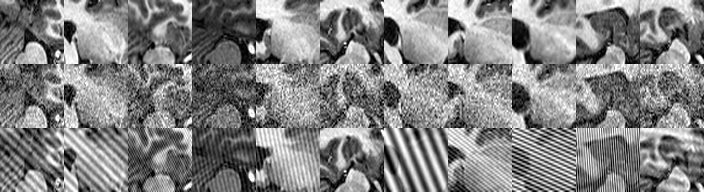
\includegraphics[width=\linewidth]{Graphics/datasets/datasets_hippo_augmented.png}\\
    \vspace{5pt}
    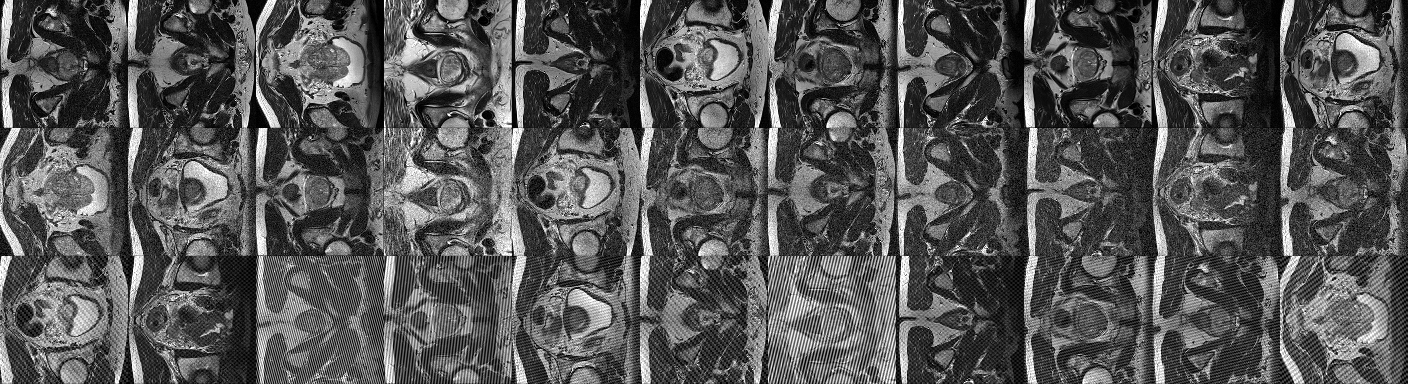
\includegraphics[width=\linewidth]{Graphics/datasets/datasets_prostate_all_augmented_highRes.png}
    \caption{Top 3: Examples from the hippocampus dataset we used. Bottom 3: Examples from the prostate datasets we used. For each 3: from top to bottom: Original from \autocite{Antonelli:2022:MedSegmentationDecatlon}, augmented with noise, augmented with spikes. We used the same noise and spike functions as here for the other datasets we generated for our test series, where only parts were augmented. However, we used different noise and spike functions for the hippocampus and prostate, as we wanted to achieve a sufficient drop in performance for our ground truth model.}
    \label{fig:augemented:datasets:augemented_hippo_prostate}
\end{figure}

%%% --- inputs ---
\subsection{Backbone-NCA on Hippocampus}
\label{experiments:03.1.0:backbone_hippo:intro}
In this section, we come to our most commonly used setup and the most comprehensive results. 
As first setup for the robustness test, we choose the BackboneNCA (\autoref{methods:NCA:Models}) and the hippocampus dataset with spike and random noise augmentations as they have just been presented.

First, we will see in \autoref{experiments:03.1.1:backbone_hippo:spike_noise} that the DiceBceNQM improves the robustness to radiological noise compared to the DiceBCE 
by up to 7 points on the Dice when artifacts were sparse (''0.01'') in the dataset, and by up to 15 points on the Dice when no artifacts were present in the training dataset, and also leads to no degradation in all other tests in this setup.

In the subsequent parts, we present several approaches to improve this setup further. Of particular note are the speedup achieved by using pretrained models (\autoref{experiments:03.1.2:backbone_hippo:pretrained}) and a minimum stacksize of 2 (\autoref{experiments:03.1.3:backbone_hippo:stackSize}). With both approaches, we did not notice any loss of robustness gain due to the DiceBceNQM.

Then we introduce the hyperparameter alpha ($\alpha$) in \autoref{experiments:03.1.4:backbone_hippo:alpha}, which at a value of 2.0 increases robustness furthermore compared to DiceBceNQM without alpha by up to 4 points on the Dice.
Finally, in \autoref{experiments:03.1.x:FurtherNQMLosses} we come to the testing of alternative nonlinear loss functions with NQM, where especially the sqrtNQM (\autoref{experiments:03.1.7:backbone_hippo:sqrtNQM}) is a promising candidate, mainly because this loss shows equivalent robustness improvements, but should converge faster. However, speed tests in this regard were not part of this work.

%%% --- inputs ---
\input{content/experiments/03_Robustness_Improving/03.1_Backbone_and_Hippocampus/03.1.1_Augmented_spikesAndNoise}
\input{content/experiments/03_Robustness_Improving/03.1_Backbone_and_Hippocampus/03.1.2_pretrained}
\input{content/experiments/03_Robustness_Improving/03.1_Backbone_and_Hippocampus/03.1.w_Hyperparameters}
\input{content/experiments/03_Robustness_Improving/03.1_Backbone_and_Hippocampus/03.1.x_FurtherNQMLosses} % subsection
\subsection{Med-NCA on Prostate}
\label{experiments:03.2.0:med_prost:intro}
After \autoref{experiments:03.1.1:backbone_hippo:spike_noise} showed that the robustness of the backbone model on the hippocampus dataset can be improved with the DiceBceNQM, we tested whether this could be transferred to a more complex model and a different dataset. We used the Med-NCA (\autoref{methods:NCA:Med-NCA}) and the medical segmentation decathlon prostate dataset \cite{Antonelli:2022:MedSegmentationDecatlon}.\\
For this purpose, we artificially augmented the prostate dataset, as well as the hippocampus dataset before, with spikes and random noise, as described in \autoref{experiments:03.0:Intro}. We also generated a series of perturbed datasets with domain shifts for the prostate dataset. Again, as described in \autoref{experiments:03.0:Intro}. \\
However, this led to much more mixed results than the backbone NCA on the hippocampus dataset (\autoref{experiments:03.1.1:backbone_hippo:spike_noise}), as we will see in this subsection.
In all cohorts, there were some training datasets where DiceBceNQM provided significant improvements over DiceBCE alone, but also some datasets where there was significant degradation. 
In the augmentations, which initially showed enormous scatter on the fist training setup, the differences between DiceBCE and DiceBceNQM became significantly smaller by extending the training cycle. Not only, but also to the disadvantage of DiceBceNQM. 
The results of the domain shifts can be divided into two parts. On the one hand, there were similar or even worse results on datasets where only a few samples were added, but which we could not resolve or improve.
On the other hand, there were significant improvements with the DiceBceNQM on the dataset merged from several sources, the all joined.

However, not only because of the poor adaptation to the augmented and shifted datasets, the question arises whether much simpler techniques than using the DiceBceNQM instead of the DiceBCE might achieve more significant effects, such as extending the training time (in the best case up to convergence), increasing the batch size, or even targeted or selective batch duplication. Especially regarding the optimal use of available resources, the DiceBceNQM requires a lot of graphics memory due to the multiple output generation.


%%% --- inputs ---
\input{content/experiments/03_Robustness_Improving/03.2_medNCA_and_Prostate/03.2.1_Augmented_spikesAndNoise}
\input{content/experiments/03_Robustness_Improving/03.2_medNCA_and_Prostate/03.2.2_DomainShifts}      % subsection
\subsection{Med-NCA on Hippocampus}
\label{experiments:03.3.0:med_hippo:intro_and_Augmented}
Due to the different results regarding the robustness improvement potential in \autoref{experiments:03.1.1:backbone_hippo:spike_noise} and \autoref{experiments:03.2.0:med_prost:intro}, we decided to investigate the transferability to another model \textit{and} another dataset separately. In this subsection, we will look at the transferability of the results from the hippocampus dataset to another model, the Med-NCA. In the next section, we will look at the transferability to another dataset with the same model as in \autoref{experiments:03.1.1:backbone_hippo:spike_noise}, the Backbone-NCA.

Therefor, we train a cohort on the hippocampus spike series on a pretrained model. The results can be seen in \autoref{tab:03.3.medNCA_Hippo_Spikes}. There are absolutely no differences between the DiceBCE and the DiceBceNQM with the Med-NCA. Considering that the same test with the Backbone-NCA showed apparent differences of up to +9 points (\autoref{tab:03.1.1:DiceBCE+NQM_vs_DiceBCE_on_Spike} and \autoref{tab:03.1.1:DiceBCE+NQM_vs_DiceBCE_on_Spike}), it is reasonable to assume that the Med-NCA, due to its architecture on top of the DiceBCE, leads to equivalent robustness here. This assumption is supported by the fact that the Med-NCA performed even better for domain shifts on the prostate dataset with the DiceBCE than with the DiceBceNQM ((\autoref{experiments:03.2.0:med_prost:intro}). With the one, but not negligible, exception from the all joined dataset.

Of course, validating or counter-testing this statement with other datasets is still essential, especially concerning domain shifts.

\iffalse
mean: 0.0005
mean on absoulte values: 0.0007
sum: 0.018
sum on absoulte values: 0.024
amax: 0.003
amax on absoulte values: 0.003
amin: -0.002
amin on absoulte values: 0.0

==> NO DIFFRENCES AT ALL 
... so it seams, MedNCA outperformces the DiceBceNQM in robustness allready with a diffrent technic or its improved architecture, ... 


mean: 0.0005
mean on absoulte values: 0.0007
sum: 0.018
sum on absoulte values: 0.024
amax: 0.003
amax on absoulte values: 0.003
amin: -0.002
amin on absoulte values: 0.0

==> NO DIFFRENCES AT ALL 
... so it seams, MedNCA outperformces the DiceBceNQM in robustness allready with a diffrent technic or its improved architecture, ... 
\fi
\iftable
\input{content/experiments/03_Robustness_Improving/03.1_Backbone_and_Hippocampus/tables/table_03.1.1_Aug_spike_noise}
\input{content/experiments/03_Robustness_Improving/03.3_medNCA_and_Hippocampus/tables/table_03.3_medNCA_Hippo}
\fi   % subsection
\subsection{Backbone-NCA on Prostate}
\label{experiments:03.4.0:backbone_prost:intro}
In \autoref{experiments:03.1.1:backbone_hippo:spike_noise}, it was shown that the DiceBceNQM loss can improve the robustness of the Backbone-NCA on the hippocampus dataset. In \autoref{experiments:03.2.0:med_prost:intro}, we saw unclear results regarding whether this could be transferred to a more complex model \textit{and} another dataset, so we decided to investigate this separately. In \autoref{experiments:03.3.0:med_hippo:intro_and_Augmented}, we already looked at the transferability of the results from the hippocampus dataset to another model, the Med-NCA. In this section, we want to look at the transferability to another dataset with the same model as in \autoref{experiments:03.1.1:backbone_hippo:spike_noise}. We, therefore, tested the behavior of the Backbone NCA on the prostate datasets. We tested this on both augmented data (\autoref{experiments:03.4.1:backbone_prost:Augmented}) and domain shifts (\autoref{experiments:03.4.2:Backbone_prost:DomainShifts}). 
The results of the augmentations and domain shifts were similar to those of the Med-NCA, suggesting that the prostate dataset, rather than the model, is more challenging in transferability than the hippocampus dataset, but this would need to be verified with additional datasets. In particular, the all joined dataset is (partially) worse here, which reduces the results with the Med-NCA in this respect.


%%% --- inputs ---
\input{content/experiments/03_Robustness_Improving/03.4_Backbone_and_Prostate/03.4.1_Augmented_Spikes}
\input{content/experiments/03_Robustness_Improving/03.4_Backbone_and_Prostate/03.4.2_DomainShifts}    % subsection              % section
    \chapter{Future Work}
\label{future_work}
In this thesis, we have shown that it is possible to pull the NQM inside the training circle to improve the robustness of NCAs. We developed a working approach, improved it further, identified some dead ends, and, according to the explorative approach we chose, we also identified ways for further improvement. In this chapter, we will focus on the last one.


%%%% Das wichtigste: Eigenkritik/ NQM-Kritik, Ressourcenalternativen und Grundlegendere Effekte? %%%%
First and foremost, two fundamental critical questions arise about the basic approach of including the NQM, which this thesis has not investigated.
\textbf{First,} do more fundamental effects than the NQM play a role in the functioning model-dataset constellations? For Example, a batch multiplication hidden by the output stack generation in the NQM comes into question. The loss has more information when training on the DiceBceNQM, independent of the loss itself, simply because stacksize many outputs are generated. Testing whether a model with the DiceBCE on such an output stack is as robust as with the DiceBceNQM is reasonable.
Moreover, suppose we assume that the Med-NCA brings quite similar robustness on the DiceBCE, as the Backbone-NCA does on the DiceBceNQM, because of the Med-NCA architecture. In that case, it is close to assuming that another architecture can bring more robustness than "messing around" with the loss and the NQM. E.g., by a deeper or broader hierarchy.
\textbf{Secondly,} can better effects be achieved with more straightforward or different approaches using the same resources? All conceivable alternatives come into question, first of all, simple things like increasing the batch size or the training time (in the best case until convergence) until the DiceBCE consumes as much VRAM or time as the DiceBceNQM. So far, we have primarily used the default settings of the existing framework, as far as resource-technically possible, and the models to be compared were always trained with the same parameters, regardless of resource usage. For an exploration, our approach is reasonable; for usage, the resource question is at least as important.


%%%% open strains
Furthermore, in favor of a more extensive exploration, some test strains are not finalized. Particularly concerning the strong scattering of Med-NCA. \textbf{First,} whether the stabilizations that we were able to achieve with pre-trained models and extended training time in the Med-NCA for the augmented data (\autoref{tab:03.2.1:medNCA_Prost:on_Spike}) are also transferable to the domain shifts (\autoref{experiments:03.2.2:med_prost:onDomainShifts}), has not been tested. Even if the experimental costellation and the problematic scattering results are very similar in both cases. \textbf{Secondly,} whether only a long training period totaling 3000 epochs made the difference or only using a pretrained model or both. \textbf{Thirdly,} since our approach with the Med-NCA has so far led to a stabilization of the results because they no longer scatter downwards but to no improvement in robustness, the question arises as to whether the outliers \textit{upwards} can be made usable. In particular, models that scatter strongly upwards are often positive on all test datasets (Noise 0.2, Spike 0.1, Spike 0.2). If we assume that by adding the NQM, the high-dimensional solution space forms minima in more robust solutions but at the same time becomes stupidly more complex, it is conceivable that more robust models can be found with skillful control. For example, switching from DiceBCE to DiceBceNQM at the right moment or possibly more often. 
\textbf{Fourthly,} the loss can be developed further by testing if increasing the alpha further in the linear DiceBceNQM brings additional improvement or faster convergence. In \autoref{experiments:03.1.x:FurtherNQMLosses}, we tested whether the non-linear losses work at all. To check which of all working losses converges the fastest, to minimize the training time, would be a next step there. As well as testing, if the powNQM with a higher base than 3 works well, to test cubic root or a mixture of power and root functions in the sense of powNQM -1 + sqrtNQM, we consider sensible. Moreover, since we cut the NQM to the interval $(0,1)$ before we started with the robustness tests, it would also be interesting to see if there is a performance difference in not cropping.


%%%% Alternativen zu NQM als loss
Beyond that, we see further alternatives we did not touch at all but are worth noting.
\textbf{First,} instead of making the NQM usable by integrating it into the loss, another approach would be to use a periodic duplication of the volumes an intermediate model performs poorly on in the sence of the NQM. 
\textbf{Secondly,} since the NQM alone does not work as a loss because the label is not taken into account, the NQM could be further modified, by using the variance over the output-label-difference, instead of using only the variance over the outputs.
    \chapter{Conclusion}
\label{conclusions}
% Teil #1 – Worum geht es?                       = Fragestellung 
%                                                = 1. Die Erklärung der Problemstellung 
%                                                = die Fragestellung und generelle Zielsetzung deiner Abschlussarbeit
%                                                = Problemstatement
%% Einstieg + Zusammenfassung
%
% Einstieg %
In this thesis, we explored whether the NQM can be used inside the training circle to improve the robustness of an NCA; we developed a working approach, improved it, and opened ways to even further improvements.
NCAs are lightweight neural models that are promising for providing access to state-of-the-art machine leaning medical imaging in low-resource environments. Prevailing large-scale segmentation models, primarily based on U-Nets, often cannot be used there, as they require a much more expensive infrastructure \cite{kalkhof:2023:M3D-NCA}. 
Improving robustness is one of the main challenges machine learning is facing nowadays \cite{Yan:2019:DomainShiftsInMedSeg, Zhou:2023:DomainGeneralization_alsoAugmentation}, and is crucial for the medical sector since people's health is at stake. 
The NQM, a variance-based quality metric, has been developed by \cite{kalkhof:2023:M3D-NCA} to indicate an NCA's stability and detect failure cases. Therefore, the question arouse, if the NQM can also be used to improve the robustness of an NCA, which this thesis has investigated.


% Teil #2 – Wie hast du das Thema bearbeitet?    = Methoden      
%                                                = 2. Inwiefern der Ansatz anders ist zu bestehenden und was die Intuition ist 
%                                                = Welche Methodik wurde wie angewendet? 
%                                                = Hypothesen und verwendete Methoden
%%%% Zusammenfassung/ Übersicht der Arbeit %%%%%
% Grundlagen, Datensatzgenerirungen, 
The NQM uses the stochastic properties of NCAs. It measures the normalized variance over different outputs generated on the same input and thus provides a measure of the quality of an NCA. The NQM, therefore, has no application for most other machine learning approaches, as these are mostly deterministic.
As core approach, we chose to implement the NQM as an extension of an existing loss function since the NQM is constructed as a metric that is optimal when it is minimal (\autoref{experiments:01.0:Into}). Thus, we consider this approach as native to the machine learning cycle in the sense that the loss is minimized natively in the machine learning cycle. 
We have chosen to extend an existing loss because the NQM alone is not suitable for minimization due to the lack of relativization to the label, i.e., the NQM is minimal if the label is maximal, which contradicts the primary requirements of segmentation, namely to predict a label, as correctly as possible, that is, in general, a subset of the input.
That way, we developed an additive and linear weighted NQM loss, the DiceBceNQM, and a group of non-linear ones and compared the performance to the standard loss of the models we used, the DiceBCE. We examined two hyperparameters, stacksize and alpha, and tested our approach on pretrained models as well to speed it up since the NQM needs multiple outputs, and this slows down training.
Concerning robustness, we investigated our approach on two segmentation NCAs, the Backbone-NCA and the Med-NCA. For both, we tested for domain shifts as well as for radiological noise. To do so, we augmented two medical datasets with spikes and random noise, the hippocampus dataset and the prostate dataset from the medical image segmentation decathlon \cite{Antonelli:2022:MedSegmentationDecatlon}. We also used this prostate dataset as a base to simulate domain shifts, together with four other prostate datasets. We generated seven series of datasets with 27 datasets together for our robustness tests.

% Teil #3 – Was sind die wichtigsten Ergebnisse? = Ergebnisse    
%                                                = 3. Was genau damit erreicht wurde, insgesamt, mit Präsentation der Ergebnisse 
%                                                = Was sind die wichtigsten Ergebnisse?
%%% Ergebnisse
The robustness improvement results were clearly successful on the Backbone-NCA with augmentations on the hippocampus dataset \autoref{experiments:03.1.1:backbone_hippo:spike_noise}. There our additive and linear weighted variant of our NQM losses, the DiceBceNQM, improves the robustness against radiological perturbations by up to 15 points on Dice. With this model and dataset, we have also shown several possible and already working ways to improve the approach further. Since the output generation for the NQM is very resource-intensive, especially regarding VRAM usage and computation time. We showed, that doing a post-training with the DiceBceNQM on models pretrained on the DiceBCE, leads to equivalent effects, but speeds up training a lot (\autoref{experiments:03.1.2:backbone_hippo:pretrained}). As well as a minimum stacksize of two, that also reduces the extensive VRAM usage (\autoref{experiments:03.1.3:backbone_hippo:stackSize}). 
Furthermore we could identify the sqrtNQM (\autoref{experiments:03.1.x:FurtherNQMLosses}) as a promising candidate for further improvement, as it performs equally to the DiceBceNQM, but could converge faster, as well as doubling the hyperparameter alpha showed further positive effects (\autoref{experiments:03.1.4:backbone_hippo:alpha}).

On the other hand, we have seen that transferring this to another model and another dataset is not trivial and that these positive results do not necessarily occur in other constellations (\autoref{experiments:03.2.0:med_prost:intro}, \ref{experiments:03.3.0:med_hippo:intro_and_Augmented}, \ref{experiments:03.4.0:backbone_prost:intro}). This was least problematic in the case of the Med-NCA on the hippocampus dataset, where there were no changes at all. For the other ones on the other hand, we faced very widely scattered results in our test series. For the worst case, the Med-NCA on the prostate dataset, -7 to +14 on Dice for augmentations and -16 to +7 for domain shifts. However, in the end, we were able to stabilize the results for the Med-NCA and the prostate dataset for the augmentations by using pretraind models and extensively extending the training time. Due to the similar problems in the other settings, we assume it is also possible to stabilize our approach for these. However, for augmentations, the results on the Med-NCA on the prostate dataset did stabilize to -2 to +5. For the average of our test cases in this setting, using the DiceBceNQM does not bring any improvements but also no deteriorations. Therefore, our approach is at least stable there.
With our test, the scattering in results was limited to the dataset, not the model. Therefore, we assume the dataset is more challenging, which is reasonable as it contains significantly fewer samples -- 394 3D volumes for the hippocampus and only 48 for the prostate.
Furthermore, it should be emphasized that our approach on the merged dataset on the Med-NCA achieves a significant robustness increase of up to +7 on Dice for one source dataset without becoming negative on any other datasets (\autoref{experiments:03.2.2:med_prost:onDomainShifts}). This is a positive exception for this more powerful model and more challenging dataset and is definitely worth pursuing. 


% Future Works %
In \autoref{future_work}, we have discussed fundamental criticisms of our approach, pointed out alternatives, as well as open threads in our explorations and opportunities to further develop our approach.


%%%%%%%%%%%%
Overall, our results show that integrating the NQM into the loss is a powerful tool to improve the robustness of NCAs for medical image segmentation, especially regarding disturbed data and merged datasets from multiple domains. We developed a working approach, improved it, and opened ways for further improvements.
}
% \include{} --> \clearpage after(!) 
% \input{}    --> no \clearpage after

%\nocite{*}  % forces all bibliography entries to be shown
\printbibliography

% \newgeometry{left=0.5cm,bottom=0.5cm} % works, but does not look so nice
\appendix
\chapter{Tables}
\label{Tables}
The tables, that appear in the text are not repreated here as well.


In order to get as broad a picture as possible, we trained one model for each variation of our loss functions that we tested on each data set of at least one series of data sets (\autoref{experiments:03.0:Intro}). We then cross-checked these models on all data sets in the series.\\
In the tables, the models on which training was performed are indexed by the two most left rows. The data sets on which testing was performed are indexed by the remaining rows.


%%% experiments 03.1. %%%
\section{experiments \autoref{experiments:03.1.0:backbone_hippo:intro}}
% \begin{table}%[H]
    \centering
    \begin{tabular}{ll!{\vrule width 1.3pt}llllll}
        \toprule
        \multicolumn{2}{c!{\vrule width 1.3pt}}{model} &
        \multicolumn{5}{c}{\textbf{test dataset} (Dice $\uparrow$)}\\\midrule
        {\bfseries train loss} & \textbf{train set} & original & Spike 1.0 & Spike 0.3 & Spike 0.2 & Spike 0.1 & Spike 0.01\\\midrule[1.3pt]
        % ---
        DiceBCE     & original      & 0.879 & 0.574 & 0.793 & 0.791 & 0.841 & 0.880\\
        DiceBceNQM  & original      & 0.881 & 0.661 \textbf{+.09} & 0.812 +.02 & 0.811 +.02 & 0.858 +.02 & 0.881\\\rowcolor{BG}
        DiceBCE     & Spike 1.0     & 0.874 & 0.823 & 0.870 & 0.871 & 0.872 & 0.874\\\rowcolor{BG}
        DiceBceNQM  & Spike 1.0     & 0.873 & 0.814 -.01 & 0.870 & 0.866 -.01 & 0.872 & 0.873\\
        DiceBCE     & Spike 0.3     & 0.878 & 0.757 & 0.856 & 0.862 & 0.875 & 0.878\\
        DiceBceNQM  & Spike 0.3     & 0.879 & 0.769 +.01 & 0.861 +.01 & 0.864 & 0.873 & 0.878\\\rowcolor{BG}
        DiceBCE     & Spike 0.2     & 0.878 & 0.731 & 0.839 & 0.858 & 0.866 & 0.878\\\rowcolor{BG}
        DiceBceNQM  & Spike 0.2     & 0.879 & 0.744 +.01 & 0.837 & 0.864 +.01 & 0.868 & 0.879\\
        DiceBCE     & Spike 0.1     & 0.879 & 0.730 & 0.844 & 0.856 & 0.873 & 0.879\\
        DiceBceNQM  & Spike 0.1     & 0.880 & 0.755 +.03 & 0.851 +.01 & 0.866 +.01 & 0.874 & 0.880\\\rowcolor{BG}
        DiceBCE     & Spike 0.01    & 0.880 & 0.615 & 0.802 & 0.820 & 0.848 & 0.879\\\rowcolor{BG}
        DiceBceNQM  & Spike 0.01    & 0.880 & 0.685 \textbf{+.07} & 0.827 +.02 & 0.834 +.01 & 0.856 +.01 & 0.879\\\bottomrule
    \end{tabular}
    \caption{Backbone-NCA, hippocampus dataset \textbf{Augmented with Spikes} (\autoref{experiments:03.1.1:backbone_hippo:spike_noise}): Using the DiceBceNQM improves robustness in this setting without having any adverse effects. First and foremost, a model trained on the original dataset with the DiceBceNQM becomes much more robust on the Spiked Dataset than if trained on the DiceBCE alone.}
    \label{tab:03.1.1:DiceBCE+NQM_vs_DiceBCE_on_Spike}
\end{table}
\begin{table}%[H]
    \centering
    \begin{tabular}{ll!{\vrule width 1.3pt}llllll}
        \toprule
        \multicolumn{2}{c!{\vrule width 1.3pt}}{model} &
        \multicolumn{5}{c}{\textbf{test dataset} (Dice $\uparrow$)}\\\midrule
        {\bfseries train loss} & \textbf{train set} & original & Noise 1.0 & Noise 0.3 & Noise 0.2 & Noise 0.1 & Noise 0.01\\\midrule[1.3pt]
        % ---
        DiceBCE     & original            & 0.880 & 0.549 & 0.798 & 0.823 & 0.859 & 0.880\\
        DiceBceNQM  & original            & 0.881 & 0.703 \textbf{+.15} & 0.839 +.04 & 0.852 +.03 & 0.871 +.01 & 0.881\\\rowcolor{BG}
        DiceBCE     & Noise 1.0     & 0.869 & 0.859 & 0.867 & 0.868 & 0.869 & 0.869\\\rowcolor{BG}
        DiceBceNQM  & Noise 1.0     & 0.867 & 0.863 & 0.865 & 0.867 & 0.866 & 0.867\\
        DiceBCE     & Noise 0.3     & 0.875 & 0.850 & 0.867 & 0.871 & 0.873 & 0.875\\
        DiceBceNQM  & Noise 0.3     & 0.879 & 0.854 & 0.873 +.01 & 0.876 +.01 & 0.877 & 0.879\\\rowcolor{BG}
        DiceBCE     & Noise 0.2     & 0.880 & 0.842 & 0.870 & 0.875 & 0.878 & 0.881\\\rowcolor{BG}
        DiceBceNQM  & Noise 0.2     & 0.881 & 0.850 +.01 & 0.873 & 0.876 & 0.879 & 0.881\\
        DiceBCE     & Noise 0.1     & 0.878 & 0.839 & 0.868 & 0.873 & 0.876 & 0.878\\
        DiceBceNQM  & Noise 0.1     & 0.881 & 0.844 +.01 & 0.871 & 0.876 & 0.878 & 0.881\\\rowcolor{BG}
        DiceBCE     & Noise 0.01    & 0.877 & 0.812 & 0.859 & 0.867 & 0.873 & 0.877\\\rowcolor{BG}
        DiceBceNQM  & Noise 0.01    & 0.879 & 0.832 +.02 & 0.867 +.01 & 0.871 & 0.876 & 0.879\\\bottomrule
    \end{tabular}
    \caption{Backbone-NCA, hippocampus dataset \textbf{Augmented with Noise} (\autoref{experiments:03.1.1:backbone_hippo:spike_noise}): Using the DiceBceNQM improves robustness in this setting without having any adverse effects. First and foremost, a model trained on the original dataset with the DiceBceNQM becomes much more robust on the Noised Dataset than if trained on the DiceBCE alone.}
    \label{tab:03.1.1:DiceBCE+NQM_vs_DiceBCE_on_Noise}
\end{table} % in text
% \begin{table}[H]
    \centering
    \begin{tabular}{cl!{\vrule width 1.3pt}llllll}
        \toprule
        \multicolumn{2}{c!{\vrule width 1.3pt}}{model} &
        \multicolumn{5}{c}{\textbf{test dataset} (Dice $\uparrow$)}\\\midrule
        {\bfseries pretrained} & \textbf{train set} & original & Spike 1.0 & Spike 0.3 & Spike 0.2 & Spike 0.1 & Spike 0.01\\\midrule[1.3pt]
        % ---
        no  & original           & 0.881 & 0.662 & 0.812 & 0.811 & 0.858 & 0.881                            \\
        yes & original           & 0.879 & 0.639 -.02 & 0.802 -.01 & 0.801 -.01 & 0.857 & 0.879             \\\rowcolor{BG}
        no  & Spike 1.0          & 0.867 & 0.817 & 0.864 & 0.863 & 0.865 & 0.866                            \\\rowcolor{BG}
        yes & Spike 1.0          & 0.874 +.01 & 0.812 & 0.871 +.01 & 0.867 & 0.872 +.01 & 0.874 +.01        \\
        no  & Spike 0.3          & 0.874 & 0.750 & 0.853 & 0.859 & 0.870 & 0.875                            \\
        yes & Spike 0.3          & 0.872 & 0.757 +.01 & 0.858 +.01 & 0.859 & 0.868 & 0.872                  \\\rowcolor{BG}
        no  & Spike 0.2          & 0.878 & 0.751 & 0.843 & 0.863 & 0.869 & 0.878                            \\\rowcolor{BG}
        yes & Spike 0.2          & 0.879 & 0.727 -.02 & 0.830 -.01 & 0.862 & 0.869 & 0.879                  \\
        no  & Spike 0.1          & 0.875 & 0.754 & 0.849 & 0.860 & 0.869 & 0.876                            \\
        yes & Spike 0.1          & 0.875 & 0.735 -.02 & 0.842 -.01 & 0.855 -.01 & 0.866 & 0.875             \\\rowcolor{BG}
        no  & Spike 0.01         & 0.877 & 0.644 & 0.801 & 0.811 & 0.852 & 0.877                            \\\rowcolor{BG}
        yes & Spike 0.01         & 0.878 & 0.681 \textbf{+.04} & 0.816 +.01 & 0.833 +.02 & 0.861 +.01 & 0.877        \\\bottomrule
    \end{tabular}
    \caption{\textbf{Pretrained Models} (\autoref{experiments:03.1.2:backbone_hippo:pretrained}): Comparrison between pretrained models and full trained ones. For the pretrained models, we used the DiceBCE for the first 500 epochs, since it is faster, and trained after that on the DiceBceNQM for additional 100 epochs. For the not pretrained models we trained full 600 epochs on DiceBceNQM as baseline for the pretrained.\\
    The pretrained models are as good, as the full trained ones. Therefor they can be used to speed up training.}
    \label{tab:3.1.2:DiceBCE+NQM:Pretrained}  
\end{table} % in text
\begin{table}[H]
    \centering
    \begin{tabular}{cl!{\vrule width 1.3pt}llllll}
        \toprule
        \multicolumn{2}{c!{\vrule width 1.3pt}}{model} &
        \multicolumn{5}{c}{\textbf{test dataset} (Dice $\uparrow$)}\\\midrule
        {\bfseries Stacksize} & \textbf{train set} & original & Spike 1.0 & Spike 0.3 & Spike 0.2 & Spike 0.1 & Spike 0.01\\\midrule[1.3pt]
        % ---
        3 & original    & 0.881 & 0.611 & 0.798 & 0.799 & 0.856 & 0.881\\\rowcolor{BG}
        3 & Spike 0.3   & 0.878 & 0.782 & 0.868 & 0.863 & 0.873 & 0.877\\\rowcolor{BG}
        6 & Spike 0.3   & 0.880 & 0.788 +.01 & 0.864 & 0.865 & 0.875 & 0.879\\
        3 & Spike 0.2   & 0.876 & 0.728 & 0.832 & 0.860 & 0.868 & 0.876\\
        6 & Spike 0.2   & 0.879 & 0.743 +.02 & 0.839 +.01 & 0.862 & 0.867 & 0.879\\\rowcolor{BG}
        3 & Spike 0.1   & 0.880 & 0.753 & 0.856 & 0.862 & 0.875 & 0.880\\\rowcolor{BG}
        6 & Spike 0.1   & 0.877 & 0.738 -.02 & 0.848 -.01 & 0.859 & 0.870 -.01 & 0.877\\\bottomrule
    \end{tabular}
    \caption{\textbf{Higher Stacksize} (\autoref{experiments:03.1.3:backbone_hippo:stackSize}): Comparrison between stacksize 3 and stacksize 6. Model from first line is traind on Dice BCE for comparison. For the other models here, the trainloss is the DiceBceNQM, but with diffrent stackSize.\\
    A higher stacksize does not take any effekt, even though it is very expensive in computation time. All models are trained with a batchsize of 16, since the VRAM need with a stacksize of 6 was to high otherwise.}
    \label{tab:3.1.3:higherStacksize}
\end{table}

\begin{table}[H]
    \centering
    \begin{tabular}{cl!{\vrule width 1.3pt}llllll}
        \toprule
        \multicolumn{2}{c!{\vrule width 1.3pt}}{model} &
        \multicolumn{5}{c}{\textbf{test dataset} (Dice $\uparrow$)}\\\midrule
        {\bfseries Stacksize} & \textbf{train set} & original & Spike 1.0 & Spike 0.3 & Spike 0.2 & Spike 0.1 & Spike 0.01\\\midrule[1.3pt]
        % ---
        3 & original        & 0.881 & 0.662 & 0.812 & 0.811 & 0.858 & 0.881                           \\
        2 & original        & 0.882 & 0.645 -.02 & 0.801 -.01 & 0.809 & 0.853 -.01 & 0.883            \\\rowcolor{BG}
        3 & Spike1.0  & 0.867 & 0.817 & 0.864 & 0.863 & 0.865 & 0.866                           \\\rowcolor{BG}
        2 & Spike1.0  & 0.872 +.01 & 0.825 +.01 & 0.867 & 0.867 & 0.870 +.01 & 0.872 +.01       \\
        3 & Spike0.3  & 0.874 & 0.750 & 0.853 & 0.859 & 0.870 & 0.875                           \\
        2 & Spike0.3  & 0.876 & 0.756 +.01 & 0.854 & 0.858 & 0.871 & 0.875                      \\\rowcolor{BG}
        3 & Spike0.2  & 0.878 & 0.751 & 0.843 & 0.863 & 0.869 & 0.878                           \\\rowcolor{BG}
        2 & Spike0.2  & 0.878 & 0.737 -.01 & 0.835 -.01 & 0.861 & 0.864 -.01 & 0.878            \\
        3 & Spike0.1  & 0.875 & 0.754 & 0.849 & 0.860 & 0.869 & 0.876                           \\
        2 & Spike0.1  & 0.880 +.01 & 0.765 +.01 & 0.858 +.01 & 0.865 +.01 & 0.875 +.01 & 0.880  \\\rowcolor{BG}
        3 & Spike0.01 & 0.877 & 0.644 & 0.801 & 0.811 & 0.852 & 0.877                           \\\rowcolor{BG}
        2 & Spike0.01 & 0.881 & 0.659 +.02 & 0.816 +.01 & 0.823 +.01 & 0.861 +.01 & 0.881       \\\bottomrule
    \end{tabular}
    \caption{\textbf{Smaller Stacksize} (\autoref{experiments:03.1.3:backbone_hippo:stackSize}): Comparrison between stacksize 3 and stacksize 2. Models are trained on the DiceBceNQM, but with diffrent stackSize.\\
    A stacksize of 2 is as good as a stacksize of 3, even though a higher stacksize is more expensive in computation time and VRAM.}
    \label{tab:3.1.3:smallerStacksize}
\end{table}
\begin{table}[H]
    \centering
    \begin{tabular}{cl!{\vrule width 1.3pt}llllll}
        \toprule
        \multicolumn{2}{c!{\vrule width 1.3pt}}{model} &
        \multicolumn{5}{c}{\textbf{test dataset} (Dice $\uparrow$)}\\\midrule
        \textbf{alpha} & \textbf{train set} & original & spike 1.0 & spike 0.3 & spike 0.2 & spike 0.1 & spike 0.01\\\midrule[1.3pt]
        % ---
        1.0 & original     & 0.881 & 0.662 & 0.812 & 0.811 & 0.858 & 0.881\\
        0.5 & original     & 0.881 & 0.636 \textbf{-.03} & 0.808 & 0.790 -.02 & 0.850 -.01 & 0.880\\
        2.0 & original     & 0.879 & 0.672 +.01 & 0.815 & 0.821 +.01 & 0.858 & 0.879\\\rowcolor{BG}
        1.0 & Spike 1.0    & 0.867 & 0.817 & 0.864 & 0.863 & 0.865 & 0.866\\\rowcolor{BG}
        0.5 & Spike 1.0    & 0.873 +.01 & 0.805 -.01 & 0.868 & 0.866 & 0.871 +.01 & 0.874 +.01\\\rowcolor{BG}
        2.0 & Spike 1.0    & 0.869 & 0.814 & 0.866 & 0.863 & 0.868 & 0.869\\
        1.0 & Spike 0.3    & 0.874 & 0.750 & 0.853 & 0.859 & 0.870 & 0.875\\
        0.5 & Spike 0.3    & 0.876 & 0.745 -.01 & 0.854 & 0.862 & 0.870 & 0.877\\
        2.0 & Spike 0.3    & 0.875 & 0.771 +.02 & 0.858 +.01 & 0.861 & 0.871 & 0.875\\\rowcolor{BG}
        1.0 & Spike 0.2    & 0.878 & 0.751 & 0.843 & 0.863 & 0.869 & 0.878\\\rowcolor{BG}
        0.5 & Spike 0.2    & 0.878 & 0.739 -.01 & 0.842 & 0.863 & 0.867 & 0.878\\\rowcolor{BG}
        2.0 & Spike 0.2    & 0.878 & 0.738 -.01 & 0.835 -.01 & 0.862 & 0.870 & 0.878\\
        1.0 & Spike 0.1    & 0.875 & 0.754 & 0.849 & 0.860 & 0.869 & 0.876\\
        0.5 & Spike 0.1    & 0.879 & 0.762 +.01 & 0.850 & 0.860 & 0.875 +.01 & 0.879\\
        2.0 & Spike 0.1    & 0.874 & 0.759 +.01 & 0.846 & 0.856 & 0.870 & 0.875\\\rowcolor{BG}
        1.0 & Spike 0.01   & 0.877 & 0.644 & 0.801 & 0.811 & 0.852 & 0.877\\\rowcolor{BG}
        0.5 & Spike 0.01   & 0.880 & 0.639 -.01 & 0.808 +.01 & 0.806 -.01 & 0.856 & 0.880\\\rowcolor{BG}
        2.0 & Spike 0.01   & 0.879 & 0.686 \textbf{+.04} & 0.826 +.02 & 0.846 \textbf{+.03} & 0.865 +.01 & 0.879\\\bottomrule
    \end{tabular}
    \caption{\textbf{DiceBceNQM with different alphas} (\autoref{experiments:03.1.4:backbone_hippo:alpha}): The standard we used for all other experiments for $\alpha$ is $1.0$. So the diffrences shown are with respect to the models trained with $\alpha=1.0$ on the same train dataset.\\ 
    An $\alpha$ of $2.0$ leads to more robust models here.}
    \label{tab:3.1.4:alpha}
\end{table}
\begin{table}[H]
    \centering
    \begin{tabular}{ll!{\vrule width 1.3pt}llllll}
        \toprule
        \multicolumn{2}{c!{\vrule width 1.3pt}}{model} &
        \multicolumn{5}{c}{\textbf{test dataset} (Dice $\uparrow$)}\\\midrule
        {\bfseries train loss} & \textbf{train set} & original & spike 1.0 & spike 0.3 & spike 0.2 & spike 0.1 & spike 0.01\\\midrule[1.3pt]
        % ---
        DiceBceNQM     & original     & 0.881 & 0.662 & 0.812 & 0.811 & 0.858 & 0.881\\
        logNQM base 2  & original     & 0.878 & 0.609 \textbf{-.05} & 0.800 -.01 & 0.797 -.01 & 0.847 -.01 & 0.877\\
        logNQM base e  & original     & 0.879 & 0.624 \textbf{-.04} & 0.803 -.01 & 0.795 -.02 & 0.848 -.01 & 0.879\\
        logNQM base 3  & original     & 0.881 & 0.576 \textbf{-.09} & 0.797 -.02 & 0.789 -.02 & 0.842 -.02 & 0.881\\
        logNQM base 10 & original     & 0.882 & 0.625 \textbf{-.04} & 0.810 & 0.805 -.01 & 0.854 & 0.882\\\rowcolor{BG}
        DiceBceNQM     & Spike 1.0    & 0.867 & 0.817 & 0.864 & 0.863 & 0.865 & 0.866\\\rowcolor{BG}
        logNQM base 2  & Spike 1.0    & 0.869 & 0.813 & 0.865 & 0.864 & 0.867 & 0.869\\\rowcolor{BG}
        logNQM base e  & Spike 1.0    & 0.873 +.01 & 0.822 +.01 & 0.869 +.01 & 0.868 +.01 & 0.871 +.01 & 0.872 +.01\\\rowcolor{BG}
        logNQM base 3  & Spike 1.0    & 0.870 & 0.831 +.01 & 0.866 & 0.866 & 0.869 & 0.870\\\rowcolor{BG}
        logNQM base 10 & Spike 1.0    & 0.870 & 0.811 -.01 & 0.864 & 0.864 & 0.867 & 0.870\\
        DiceBceNQM     & Spike 0.3    & 0.874 & 0.750 & 0.853 & 0.859 & 0.870 & 0.875\\
        logNQM base 2  & Spike 0.3    & 0.875 & 0.747 & 0.852 & 0.859 & 0.869 & 0.874\\
        logNQM base e  & Spike 0.3    & 0.878 & 0.783 \textbf{+.03} & 0.861 +.01 & 0.864 +.01 & 0.874 & 0.878\\
        logNQM base 3  & Spike 0.3    & 0.877 & 0.756 +.01 & 0.859 +.01 & 0.862 & 0.873 & 0.877\\
        logNQM base 10 & Spike 0.3    & 0.877 & 0.774 +.02 & 0.863 +.01 & 0.862 & 0.872 & 0.877\\\rowcolor{BG}
        DiceBceNQM     & Spike 0.2    & 0.878 & 0.751 & 0.843 & 0.863 & 0.869 & 0.878\\\rowcolor{BG}
        logNQM base 2  & Spike 0.2    & 0.879 & 0.752 & 0.844 & 0.862 & 0.869 & 0.879\\\rowcolor{BG}
        logNQM base e  & Spike 0.2    & 0.873 -.01 & 0.725 \textbf{-.03} & 0.826 -.02 & 0.857 -.01 & 0.862 -.01 & 0.872 -.01\\\rowcolor{BG}
        logNQM base 3  & Spike 0.2    & 0.879 & 0.741 -.01 & 0.837 -.01 & 0.862 & 0.868 & 0.879\\\rowcolor{BG}
        logNQM base 10 & Spike 0.2    & 0.877 & 0.735 -.02 & 0.836 -.01 & 0.857 -.01 & 0.864 -.01 & 0.877\\
        DiceBceNQM     & Spike 0.1    & 0.875 & 0.754 & 0.849 & 0.860 & 0.869 & 0.876\\
        logNQM base 2  & Spike 0.1    & 0.876 & 0.744 -.01 & 0.847 & 0.860 & 0.869 & 0.877\\
        logNQM base e  & Spike 0.1    & 0.877 & 0.746 -.01 & 0.850 & 0.854 -.01 & 0.871 & 0.877\\
        logNQM base 3  & Spike 0.1    & 0.880 +.01 & 0.751 & 0.851 & 0.865 +.01 & 0.874 +.01 & 0.880\\
        logNQM base 10 & Spike 0.1    & 0.876 & 0.742 -.01 & 0.842 -.01 & 0.857 & 0.869 & 0.875\\\rowcolor{BG}
        DiceBceNQM     & Spike 0.01   & 0.877 & 0.644 & 0.801 & 0.811 & 0.852 & 0.877\\\rowcolor{BG}
        logNQM base 2  & Spike 0.01   & 0.878 & 0.674 \textbf{+.03} & 0.830 \textbf{+.03} & 0.835 +.02 & 0.857 +.01 & 0.878\\\rowcolor{BG}
        logNQM base e  & Spike 0.01   & 0.877 & 0.644 & 0.809 +.01 & 0.824 +.01 & 0.852 & 0.877\\\rowcolor{BG}
        logNQM base 3  & Spike 0.01   & 0.878 & 0.627 -.02 & 0.798 & 0.803 -.01 & 0.851 & 0.877\\\rowcolor{BG}
        logNQM base 10 & Spike 0.01   & 0.876 & 0.652 +.01 & 0.811 +.01 & 0.816 & 0.848 & 0.876\\\bottomrule
    \end{tabular}
    \caption{\textbf{logNQM for diffrent bases} (\autoref{experiments:03.1.5:backbone_hippo:logNQM}): For bases 2, e, 3 and 10. linear DiceBceNQM as comparison. Only diffrences bigger round $\pm$.01 are shown (always in comparison to the top row of the block, the model trained on the DiceBce-NQM).\\Overall, the logNQM does not lead to any further improvement in robustness here.}
    \label{tab:3.1.5:logNQM}
\end{table}
\begin{table}[H]
    \centering
    \begin{tabular}{ll!{\vrule width 1.3pt}llllll}
        \toprule
        \multicolumn{2}{c!{\vrule width 1.3pt}}{model} &
        \multicolumn{5}{c}{\textbf{test dataset} (Dice $\uparrow$)}\\\midrule
        {\bfseries train loss} & \textbf{train set} & original & spike 1.0 & spike 0.3 & spike 0.2 & spike 0.1 & spike 0.01\\\midrule[1.3pt]
        % ---
        DiceBceNQM      & original     & 0.881 & 0.662 & 0.812 & 0.811 & 0.858 & 0.881\\
        powNQM base 3   & original     & 0.877 & 0.616 \textbf{-.05} & 0.809 & 0.793 -.02 & 0.853 -.01 & 0.877\\\rowcolor{BG}
        DiceBceNQM      & Spike 1.0    & 0.867 & 0.817 & 0.864 & 0.863 & 0.865 & 0.866\\\rowcolor{BG}
        powNQM base 3   & Spike 1.0    & 0.867 & 0.815 & 0.863 & 0.859 & 0.865 & 0.867\\
        DiceBceNQM      & Spike 0.3    & 0.874 & 0.750 & 0.853 & 0.859 & 0.870 & 0.875\\
        powNQM base 3   & Spike 0.3    & 0.875 & 0.768 +.02 & 0.857 & 0.861 & 0.873 & 0.875\\\rowcolor{BG}
        DiceBceNQM      & Spike 0.2    & 0.878 & 0.751 & 0.843 & 0.863 & 0.869 & 0.878\\\rowcolor{BG}
        powNQM base 3   & Spike 0.2    & 0.874 & 0.730 -.02 & 0.832 -.01 & 0.855 -.01 & 0.863 -.01 & 0.874\\
        DiceBceNQM      & Spike 0.1    & 0.875 & 0.754 & 0.849 & 0.860 & 0.869 & 0.876\\
        powNQM base 3   & Spike 0.1    & 0.879 & 0.749 -.01 & 0.855 +.01 & 0.862 & 0.871 & 0.878\\\rowcolor{BG}
        DiceBceNQM      & Spike 0.01   & 0.877 & 0.644 & 0.801 & 0.811 & 0.852 & 0.877\\\rowcolor{BG}
        powNQM base 3   & Spike 0.01   & 0.879 & 0.668 +.02 & 0.815 +.01 & 0.832 +.02 & 0.861 +.01 & 0.879\\\bottomrule
    \end{tabular}
    \caption{\textbf{powNQM} (\autoref{experiments:03.1.6:backbone_hippo:powNQM}): Linear DiceBceNQM for comparisson. Only diffrences größer round $\pm$0.01 are shown (always in comparison to row above)\\
    Overall, powNQM base 3 does not lead to any improvement.}
    \label{tab:3.1.6:powNQM}
\end{table}
\begin{table}[H]
    \centering
    \begin{tabular}{ll!{\vrule width 1.3pt}llllll}
        \toprule
        \multicolumn{2}{c!{\vrule width 1.3pt}}{model} &
        \multicolumn{5}{c}{\textbf{test dataset} (Dice $\uparrow$)}\\\midrule
        {\bfseries train loss} & \textbf{train set} & original & spike 1.0 & spike 0.3 & spike 0.2 & spike 0.1 & spike 0.01\\\midrule[1.3pt]
        % ---
        DiceBceNQM & original       & 0.881 & 0.662 & 0.812 & 0.811 & 0.858 & 0.881\\
        sqrtNQM    & original       & 0.875 -.01 & 0.694 \textbf{+.03} & 0.816 & 0.811 & 0.852 -.01 & 0.875 -.01\\\rowcolor{BG}
        DiceBceNQM & Spike 1.0      & 0.867 & 0.817 & 0.864 & 0.863 & 0.865 & 0.866\\\rowcolor{BG}
        sqrtNQM    & Spike 1.0      & 0.868 & 0.803 -.01 & 0.864 & 0.861 & 0.866 & 0.868\\
        DiceBceNQM & Spike 0.3      & 0.874 & 0.750 & 0.853 & 0.859 & 0.870 & 0.875\\
        sqrtNQM    & Spike 0.3      & 0.873 & 0.758 +.01 & 0.854 & 0.858 & 0.868 & 0.872\\\rowcolor{BG}
        DiceBceNQM & Spike 0.2      & 0.878 & 0.751 & 0.843 & 0.863 & 0.869 & 0.878\\\rowcolor{BG}
        sqrtNQM    & Spike 0.2      & 0.870 -.01 & 0.731 -.02 & 0.825 -.02 & 0.853 -.01 & 0.860 -.01 & 0.870 -.01\\
        DiceBceNQM & Spike 0.1      & 0.875 & 0.754 & 0.849 & 0.860 & 0.869 & 0.876\\
        sqrtNQM    & Spike 0.1      & 0.868 -.01 & 0.728 -.03 & 0.836 -.01 & 0.847 -.01 & 0.859 -.01 & 0.868 -.01\\\rowcolor{BG}
        DiceBceNQM & Spike 0.01     & 0.877 & 0.644 & 0.801 & 0.811 & 0.852 & 0.877\\\rowcolor{BG}
        sqrtNQM    & Spike 0.01     & 0.876 & 0.677 \textbf{+.03} & 0.811 +.01 & 0.827 +.02 & 0.855 & 0.876\\\bottomrule
    \end{tabular}
    \caption{\textbf{sqrtNQM} (\autoref{experiments:03.1.7:backbone_hippo:sqrtNQM}): Linear DiceBceNQM for comparisson. Only diffrences größer round $\pm$0.01 are shown (always in comparison to row above)\\
    Overall, the sqrtNQM leads to another small improvement.}
    \label{tab:3.1.7:sqrtNQM}
\end{table}

%%% experiments 03.2. %%%
\newpage
\section{experiments \autoref{experiments:03.2.0:med_prost:intro}}
\begin{table}[H]
    \centering
    \begin{tabular}{ll!{\vrule width 1.3pt}llllll}
        \toprule
        \multicolumn{2}{c!{\vrule width 1.3pt}}{model} &
        \multicolumn{5}{c}{\textbf{test dataset} (Dice $\uparrow$)}\\\midrule
        {\bfseries train loss} & \textbf{train set} & original & Noise 1.0 & Noise 0.3 & Noise 0.2 & Noise 0.1 & Noise 0.01\\\midrule[1.3pt]
        % ---
        DiceBCE        & original    & 0.794 & 0.519 & 0.688 & 0.790 & 0.726 & 0.794\\
        DiceBceNQM     & original    & 0.774 -.02 & 0.559 +.04 & 0.683 & 0.774 -.02 & 0.726 & 0.767 -.03\\\rowcolor{BG}
        DiceBCE        & Noise 1.0   & 0.773 & 0.777 & 0.778 & 0.757 & 0.764 & 0.767\\\rowcolor{BG}
        DiceBceNQM     & Noise 1.0   & 0.754 -.02 & 0.780 & 0.774 & 0.754 & 0.754 -.01 & 0.755 -.01\\
        DiceBCE        & Noise 0.3   & 0.826 & 0.717 & 0.782 & 0.819 & 0.821 & 0.819\\
        DiceBceNQM     & Noise 0.3   & 0.819 -.01 & 0.746 +.03 & 0.802 +.02 & 0.819 & 0.820 & 0.821\\\rowcolor{BG}
        DiceBCE        & Noise 0.2   & 0.777 & 0.616 & 0.706 & 0.772 & 0.749 & 0.778\\\rowcolor{BG}
        DiceBceNQM     & Noise 0.2   & 0.798 +.02 & 0.678 \textbf{+.06} & 0.787 \textbf{+.08} & 0.797 +.03 & 0.798 \textbf{+.05} & 0.798 +.02\\
        DiceBCE        & Noise 0.1   & 0.798 & 0.757 & 0.780 & 0.794 & 0.779 & 0.795\\
        DiceBceNQM     & Noise 0.1   & 0.817 +.02 & 0.708 \textbf{-.05} & 0.778 & 0.818 +.02 & 0.790 +.01 & 0.815 +.02\\\rowcolor{BG}
        DiceBCE        & Noise 0.01  & 0.838 & 0.754 & 0.811 & 0.836 & 0.821 & 0.833\\\rowcolor{BG}
        DiceBceNQM     & Noise 0.01  & 0.800 -.04 & 0.720 -.03 & 0.763 \textbf{-.05} & 0.799 -.04 & 0.769 \textbf{-.05} & 0.798 -.03\\\hline
        % --- 2k --- 
        2k DiceBCE     & Noise 0.01  & 0.826 & 0.766 & 0.801 & 0.829 & 0.821 & 0.832\\
        2k DiceBceNQM  & Noise 0.01  & 0.798 -.03 & 0.694 \textbf{-.07} & 0.771 -.03 & 0.796 -.03 & 0.776 -.04 & 0.796 -.04\\\bottomrule
    \end{tabular}
    \caption{Med-NCA, prostate dataset \textbf{Augmented with Noise} 1000 epochs (\autoref{experiments:03.2.1:med_prost:augmented}): Mixed and divergent result. With this setting the approach becomes unstabel. However, this could be changed with a pretrained model for spikes (\autoref{tab:03.2.1:medNCA_Prost:on_Spike:3kepochs}). For noise this experiment was not transfered to the pretrained setting in the context of this thesis.}
    \label{tab:03.2.1:medNCA_Prost:on_Noise}
\end{table} 
% \begin{table}[H]
    \centering
    \begin{tabular}{ll!{\vrule width 1.3pt}llllll}
        \toprule
        \multicolumn{2}{c!{\vrule width 1.3pt}}{model} &
        \multicolumn{5}{c}{\textbf{test dataset} (Dice $\uparrow$)}\\\midrule
        {\bfseries train loss} & \textbf{train set}& original & Spike 1.0 & Spike 0.3 & Spike 0.2 & Spike 0.1 & Spike 0.01\\\midrule[1.3pt]
        % ---
        DiceBCE        & original    & 0.787 & 0.321 & 0.684 & 0.717 & 0.790 & 0.793\\
        DiceBceNQM     & original    & 0.772 -.02 & 0.384 \textbf{+.06} & 0.665 -.02 & 0.712 -.01 & 0.776 -.01 & 0.774 -.02\\\rowcolor{BG}
        DiceBCE        & Spike 1.0   & 0.776 & 0.593 & 0.722 & 0.678 & 0.767 & 0.780\\\rowcolor{BG}
        DiceBceNQM     & Spike 1.0   & 0.740 -.04 & 0.632 +.04 & 0.653 \textbf{-.07} & 0.666 -.01 & 0.740 -.03 & 0.740 -.04\\
        DiceBCE        & Spike 0.3   & 0.791 & 0.607 & 0.683 & 0.726 & 0.798 & 0.793\\
        DiceBceNQM     & Spike 0.3   & 0.780 -.01 & 0.658 \textbf{+.05} & 0.667 -.02 & 0.737 +.01 & 0.780 -.02 & 0.781 -.01\\\rowcolor{BG}
        DiceBCE        & Spike 0.2   & 0.774 & 0.377 & 0.656 & 0.701 & 0.776 & 0.771\\\rowcolor{BG}
        DiceBceNQM     & Spike 0.2   & 0.808 +.03 & 0.503 \textbf{+.13} & 0.693 +.04 & 0.709 +.01 & 0.810 +.03 & 0.809 +.04\\
        DiceBCE        & Spike 0.1   & 0.788 & 0.392 & 0.671 & 0.712 & 0.789 & 0.794\\
        DiceBceNQM     & Spike 0.1   & 0.802 +.01 & 0.528 \textbf{+.14} & 0.684 +.01 & 0.759 +.05 & 0.800 +.01 & 0.798\\\rowcolor{BG}
        DiceBCE        & Spike 0.01  & 0.807 & 0.353 & 0.686 & 0.721 & 0.802 & 0.807\\\rowcolor{BG}
        DiceBceNQM     & Spike 0.01  & 0.790 -.02 & 0.354 & 0.674 -.01 & 0.700 -.02 & 0.789 -.01 & 0.788 -.02\\\hline
        % --- 2k ---
        2k DiceBCE    & spike 0.01  & 0.793 & 0.345 & 0.684 & 0.711 & 0.797 & 0.790\\
        2k DiceBceNQM & spike 0.01  & 0.791 & 0.347 & 0.674 -.01 & 0.700 -.01 & 0.789 -.01 & 0.791\\\bottomrule
    \end{tabular}
    \caption{Med-NCA, prostate dataset \textbf{Augmented with Spikes} 1000 epochs (\autoref{experiments:03.2.1:med_prost:augmented}): Mixed and divergent result. With this setting the approach becomes unstabel. However, this could be changed with a pretrained model (\autoref{tab:03.2.1:medNCA_Prost:on_Spike:3kepochs}).}
    \label{tab:03.2.1:medNCA_Prost:on_Spike}
\end{table} % in text
% \begin{table}[H]
    \centering
    \begin{tabular}{ll!{\vrule width 1.3pt}llllll}
        \toprule
        \multicolumn{2}{c!{\vrule width 1.3pt}}{model} &
        \multicolumn{5}{c}{\textbf{test dataset} (Dice $\uparrow$)}\\\midrule
        {\bfseries train loss} & \textbf{train set}& original & Spike 1.0 & Spike 0.3 & Spike 0.2 & Spike 0.1 & Spike 0.01\\\midrule[1.3pt]
        % ---
        DiceBce       & original    & 0.794      & 0.368      & 0.683      & 0.712      & 0.801 & 0.795      \\
        DiceBceNQM    & original    & 0.800 +.01 & 0.367      & 0.693 +.01 & 0.727 +.02 & 0.802 & 0.808 +.01 \\\rowcolor{BG}
        DiceBce       & Spike 1.0   & 0.792      & 0.639      & 0.719      & 0.713      & 0.793 & 0.789      \\\rowcolor{BG}
        DiceBceNQM    & Spike 1.0   & 0.792      & 0.636      & 0.726 +.01 & 0.723 +.01 & 0.791 & 0.796 +.01 \\
        DiceBce       & Spike 0.3   & 0.791      & 0.584      & 0.674      & 0.710      & 0.793 & 0.793      \\
        DiceBceNQM    & Spike 0.3   & 0.783 -.01 & 0.637 \textbf{+.05} & 0.670      & 0.706      & 0.789 & 0.786 -.01 \\\rowcolor{BG}
        DiceBce       & Spike 0.2   & 0.782      & 0.399      & 0.668      & 0.711      & 0.789 & 0.792      \\\rowcolor{BG}
        DiceBceNQM    & Spike 0.2   & 0.786      & 0.421 +.02 & 0.669      & 0.713      & 0.790 & 0.789      \\
        DiceBce       & Spike 0.1   & 0.799      & 0.417      & 0.677      & 0.730      & 0.803 & 0.802      \\
        DiceBceNQM    & Spike 0.1   & 0.796      & 0.399 -.02 & 0.675      & 0.707 -.02 & 0.802 & 0.796 -.01 \\\rowcolor{BG}
        DiceBce       & Spike 0.01  & 0.795      & 0.382      & 0.677      & 0.720      & 0.797 & 0.793      \\\rowcolor{BG}
        DiceBceNQM    & Spike 0.01  & 0.797      & 0.369 -.01 & 0.678      & 0.711 -.01 & 0.793 & 0.795      \\\bottomrule
    \end{tabular}
    \caption{Med-NCA, prostate dataset \textbf{Augmented with Spikes} 1000 epochs on \textbf{pretrained model} (\autoref{experiments:03.2.1:med_prost:augmented}): A lot more stable, with this number of epochs. Except for one case, the DiceBceNQM no longer makes a difference here. Therefor the approach is stable now and no longer makes things worse in this setting.}
    \label{tab:03.2.1:medNCA_Prost:on_Spike:3kepochs}
\end{table} % in text
% \begin{table}[H]
    \centering
    \begin{tabular}{ll!{\vrule width 1.3pt}lllllll}
        \toprule
        \multicolumn{2}{c!{\vrule width 1.3pt}}{model} &
        \multicolumn{5}{c}{\textbf{test dataset} (Dice $\uparrow$)}\\\midrule
        {\bfseries train loss} & \textbf{train dataset} & decath & isbi & i2cvb & ucl & all joined\\\midrule[1.3pt]
        % ---
        diceBce     & decath          & 0.793 & 0.324 & 0.243 & 0.323 & 0.301\\
        diceBceNQM  & decath          & 0.794 & 0.329 +.01 & 0.253 +.01 & 0.325 & 0.287 -.01\\\rowcolor{BG}
        diceBce     & shift 1 isbi    & 0.772 & 0.441 & 0.256 & 0.321 & 0.367\\\rowcolor{BG}
        diceBceNQM  & shift 1 isbi    & 0.767 -.01 & 0.335 \textbf{-.11} & 0.249 -.01 & 0.324 & 0.306 \textbf{-.06}\\
        diceBce     & shift 1 i2cvb   & 0.736 & 0.340 & 0.343 & 0.327 & 0.356\\
        diceBceNQM  & shift 1 i2cvb   & 0.753 +.02 & 0.196 \textbf{-.14} & 0.376 +.03 & 0.334 +.01 & 0.290 -.07\\\rowcolor{BG}
        diceBce     & shift 1 ucl     & 0.804 & 0.407 & 0.247 & 0.326 & 0.320\\\rowcolor{BG}
        diceBceNQM  & shift 1 ucl     & 0.783 -.02 & 0.321 \textbf{-.09} & 0.258 +.01 & 0.331 +.01 & 0.271 \textbf{-.05}\\
        DiceBce     & all joined      & 0.904 & 0.812 & 0.658 & 0.821 & 0.722\\
        DiceBceNQM  & all joined      & 0.903 & 0.824 +.01 & 0.684 +.03 & 0.888 \textbf{+.07} & 0.728 +.01\\\bottomrule
    \end{tabular}
    \caption{Med-NCA, \textbf{Single Domainshifts} and \textbf{all joined} (\autoref{experiments:03.2.2:med_prost:onDomainShifts}): Test on original datasets. For the all joined dataset the DiceBceNQM is significantly more robust. It is also more instable on the datasets with single volume shifts.}
    \label{tab:03.2.2:medNCA_Prost:domainShifts:OneOnOriginals}
\end{table} % in text
% \begin{table}[H]
    \centering
    \begin{tabular}{ll!{\vrule width 1.3pt}lllllll}
        \toprule
        \multicolumn{2}{c!{\vrule width 1.3pt}}{model} &
        \multicolumn{5}{c}{\textbf{test dataset} (Dice $\uparrow$)}\\\midrule
        {\bfseries train loss} & \textbf{train dataset} & decath & isbi & i2cvb & ucl & all joined\\\midrule[1.3pt]
        % ---
        diceBce     & decath         & 0.789 & 0.306 & 0.246 & 0.323 & 0.308\\
        diceBceNQM  & decath         & 0.788 & 0.333 +.03 & 0.253 +.01 & 0.325 & 0.290 -.02\\\rowcolor{BG}
        diceBce     & shift 12 isbi  & 0.838 & 0.645 & 0.331 & 0.318 & 0.516\\\rowcolor{BG}
        diceBceNQM  & shift 12 isbi  & 0.849 +.01 & 0.643 & 0.388 \textbf{+.06} & 0.319 & 0.514\\
        diceBce     & shift 8 i2cvb  & 0.852 & 0.438 & 0.578 & 0.328 & 0.459\\
        diceBceNQM  & shift 8 i2cvb  & 0.859 +.01 & 0.304 \textbf{-.13} & 0.536 -.04 & 0.323 -.01 & 0.411 -.05\\\rowcolor{BG}
        diceBce     & shift 4 ucl    & 0.781 & 0.561 & 0.280 & 0.519 & 0.505\\\rowcolor{BG}
        diceBceNQM  & shift 4 ucl    & 0.812 +.03 & 0.397 \textbf{-.16} & 0.263 -.02 & 0.557 +.04 & 0.449 \textbf{-.06}\\\bottomrule
    \end{tabular}
    \caption{Med-NCA, \textbf{Multiple Domainshifts} (\autoref{experiments:03.2.2:med_prost:onDomainShifts}): Test on Original Datasets. Even more mixed and divergent as Single Domainshifts.}
    \label{tab:03.2.2:medNCA_Prost:domainShifts:multiOnOriginals}
\end{table} % in text
%%% experiments 03.3. %%%
\newpage
\section{experiments \autoref{experiments:03.3.0:med_hippo:intro_and_Augmented}}
\begin{table}[H]
    \centering
    \begin{tabular}{ll!{\vrule width 1.3pt}llllll}
        \toprule
        \multicolumn{2}{c!{\vrule width 1.3pt}}{model} &
        \multicolumn{5}{c}{\textbf{test dataset} (Dice $\uparrow$)}\\\midrule
        {\bfseries train loss} & \textbf{train set} & original & Spike 1.0 & Spike 0.3 & Spike 0.2 & Spike 0.1 & Spike 0.01\\\midrule[1.3pt]
        % ---
        DiceBCE     & original      & 0.878 & 0.712 & 0.832 & 0.831 & 0.870 & 0.878\\
        DiceBceNQM  & original      & 0.878 & 0.712 & 0.832 & 0.831 & 0.870 & 0.878\\\rowcolor{BG}
        DiceBCE     & Spike 1.0     & 0.870 & 0.823 & 0.865 & 0.863 & 0.869 & 0.870\\\rowcolor{BG}
        DiceBceNQM  & Spike 1.0     & 0.871 & 0.824 & 0.866 & 0.864 & 0.870 & 0.871\\
        DiceBCE     & Spike 0.3     & 0.875 & 0.802 & 0.867 & 0.854 & 0.873 & 0.875\\
        DiceBceNQM  & Spike 0.3     & 0.875 & 0.801 & 0.867 & 0.855 & 0.873 & 0.876\\\rowcolor{BG}
        DiceBCE     & Spike 0.2     & 0.879 & 0.775 & 0.864 & 0.858 & 0.876 & 0.878\\\rowcolor{BG}
        DiceBceNQM  & Spike 0.2     & 0.879 & 0.773 & 0.864 & 0.860 & 0.876 & 0.879\\
        DiceBCE     & Spike 0.1     & 0.876 & 0.783 & 0.854 & 0.854 & 0.873 & 0.876\\
        DiceBceNQM  & Spike 0.1     & 0.877 & 0.784 & 0.855 & 0.855 & 0.873 & 0.877\\\rowcolor{BG}
        DiceBCE     & Spike 0.01    & 0.877 & 0.724 & 0.840 & 0.837 & 0.870 & 0.876\\\rowcolor{BG}
        DiceBceNQM  & Spike 0.01    & 0.877 & 0.727 & 0.841 & 0.837 & 0.871 & 0.876\\\bottomrule
    \end{tabular}
    \caption{Med-NCA, hippocampus dataset \textbf{Augmented with Spikes}  (\autoref{experiments:03.3.0:med_hippo:intro_and_Augmented}): Here we have absolutly no diffrences at all between the DiceBCE and the DiceBceNQM.}
    \label{tab:03.3.medNCA_Hippo_Spikes}
\end{table}

%%% experiments 03.4. %%%
\newpage
\section{experiments \autoref{experiments:03.4.0:backbone_prost:intro}}
\begin{table}[H]
    \centering
    \begin{tabular}{ll!{\vrule width 1.3pt}llllll}
        \toprule
        \multicolumn{2}{c!{\vrule width 1.3pt}}{model} &
        \multicolumn{5}{c}{\textbf{test dataset} (Dice $\uparrow$)}\\\midrule
        {\bfseries train loss} & \textbf{train set} & original & Spike 1.0 & Spike 0.3 & Spike 0.2 & Spike 0.1 & Spike 0.01\\\midrule[1.3pt]
        % ---
        DiceBCE        & original    & 0.788 & 0.277 & 0.661 & 0.717 & 0.788 & 0.787\\
        DiceBCENQM     & original    & 0.798 +.01 & 0.297 +.02 & 0.663 & 0.719 & 0.804 +.02 & 0.795 +.01\\\rowcolor{BG}
        DiceBCE        & Spike 1.0   & 0.781 & 0.656 & 0.678 & 0.788 & 0.780 & 0.777\\\rowcolor{BG}
        DiceBceNQM     & Spike 1.0   & 0.783 & 0.601 \textbf{-.06} & 0.699 +.02 & 0.757 \textbf{-.03} & 0.769 -.01 & 0.774\\
        DiceBCE        & Spike 0.3   & 0.746 & 0.295 & 0.638 & 0.706 & 0.774 & 0.768\\
        DiceBceNQM     & Spike 0.3   & 0.776 \textbf{+.03} & 0.301 +.01 & 0.654 +.02 & 0.709 & 0.771 & 0.768\\\rowcolor{BG}
        DiceBCE        & Spike 0.2   & 0.798 & 0.301 & 0.677 & 0.725 & 0.804 & 0.798\\\rowcolor{BG}
        DiceBceNQM     & Spike 0.2   & 0.785 -.01 & 0.289 -.01 & 0.672 -.01 & 0.720 -.01 & 0.785 -.02 & 0.785 -.01\\
        DiceBCE        & Spike 0.1   & 0.795 & 0.354 & 0.686 & 0.751 & 0.797 & 0.801\\
        DiceBceNQM     & Spike 0.1   & 0.815 +.02 & 0.363 +.01 & 0.697 +.01 & 0.791 \textbf{+.04} & 0.819 +.02 & 0.822 +.02\\\rowcolor{BG}
        DiceBCE        & Spike 0.01  & 0.809 & 0.326 & 0.682 & 0.731 & 0.806 & 0.811\\\rowcolor{BG}
        DiceBceNQM     & Spike 0.01  & 0.796 -.01 & 0.321 -.01 & 0.669 -.01 & 0.724 -.01 & 0.798 -.01 & 0.796 -.02\\\bottomrule
    \end{tabular}
    \caption{Backbone-NCA, prostate dataset \textbf{Augmented with Spikes} (\autoref{experiments:03.4.1:backbone_prost:Augmented}): On Pretrained Model. Mixed results, as with the Med-NCA. Even more divergent, but overall not worse.}
    \label{tab:03.4.1:Backbone_Prost:on_Spike}
\end{table}
\begin{table}[H]
    \centering
    \begin{tabular}{ll!{\vrule width 1.3pt}lllll}
        \toprule
        \multicolumn{2}{c!{\vrule width 1.3pt}}{model} &
        \multicolumn{5}{c}{\textbf{test dataset} (Dice $\uparrow$)}\\\midrule
        {\bfseries train loss} & \textbf{train dataset} & decath & isbi & i2cvb & ulc & all joined\\\midrule[1.3pt]
        % ---
        diceBce     & decath           & 0.776 & 0.427 & 0.236 & 0.313 & 0.370\\
        diceBceNQM  & decath           & 0.795 +.02 & 0.486 \textbf{+.06} & 0.254 +.02 & 0.322 +.01 & 0.383 +.01\\\rowcolor{BG}
        diceBce     & shift 1 isbi     & 0.782 & 0.541 & 0.252 & 0.327 & 0.424\\\rowcolor{BG}
        diceBceNQM  & shift 1 isbi     & 0.774 -.01 & 0.527 -.01 & 0.283 \textbf{+.03} & 0.327 & 0.402 -.02\\
        diceBce     & shift 1 i2cvb    & 0.767 & 0.354 & 0.274 & 0.332 & 0.355\\
        diceBceNQM  & shift 1 i2cvb    & 0.765 & 0.343 -.01 & 0.256 -.02 & 0.330 & 0.361 +.01\\\rowcolor{BG}
        diceBce     & shift 1 ucl      & 0.806 & 0.511 & 0.237 & 0.345 & 0.377\\\rowcolor{BG}
        diceBceNQM  & shift 1 ucl      & 0.786 -.02 & 0.483 \textbf{-.03} & 0.257 +.02 & 0.343 & 0.382 +.01\\
        DiceBce     & all joined       & 0.919 & 0.905 & 0.759 & 0.923 & 0.794\\
        DiceBceNQM  & all joined       & 0.904 -.02 & 0.894 -.01 & 0.697 \textbf{-.06} & 0.933 +.01 & 0.800 +.01\\\bottomrule
    \end{tabular}
    \caption{Backbone-NCA, \textbf{Single Domainshifts} and \textbf{all joined} (\autoref{experiments:03.4.2:Backbone_prost:DomainShifts}): Tests on original datasets. Very divergent and mixed results. But a lot less divergent then for the Med-NCA.}
    \label{tab:03.4.2:Backbone_Prost:domainShifts:OneOnOriginals}
\end{table}
\begin{table}[H]
    \centering
    \begin{tabular}{ll!{\vrule width 1.3pt}lllllll}
        \toprule
        \multicolumn{2}{c!{\vrule width 1.3pt}}{model} &
        \multicolumn{5}{c}{\textbf{test dataset} (Dice $\uparrow$)}\\\midrule
        {\bfseries train loss} & \textbf{train dataset} & decath & isbi & i2cvb & ulc & all joined\\\midrule[1.3pt]
        % ---
        diceBce     & decath          & 0.792 & 0.410 & 0.236 & 0.314 & 0.365\\
        diceBceNQM  & decath          & 0.789 & 0.497 \textbf{+.09} & 0.254 +.02 & 0.322 +.01 & 0.383 +.02\\\rowcolor{BG}
        diceBce     & shift 12 isbi   & 0.864 & 0.731 & 0.302 & 0.322 & 0.548\\\rowcolor{BG}
        diceBceNQM  & shift 12 isbi   & 0.877 +.01 & 0.714 -.02 & 0.259 \textbf{-.04} & 0.327 +.01 & 0.572 +.02\\
        diceBce     & shift 8 i2cvb   & 0.873 & 0.498 & 0.482 & 0.327 & 0.499\\
        diceBceNQM  & shift 8 i2cvb   & 0.867 -.01 & 0.428 \textbf{-.07} & 0.551 \textbf{+.07} & 0.333 +.01 & 0.494 -.01\\\rowcolor{BG}
        diceBce     & shift 4 ucl     & 0.750 & 0.659 & 0.250 & 0.681 & 0.582\\\rowcolor{BG}
        diceBceNQM  & shift 4 ucl     & 0.805 \textbf{+.06} & 0.619 \textbf{-.04} & 0.266 +.02 & 0.638 \textbf{-.04} & 0.566 -.02\\\bottomrule
    \end{tabular}
    \caption{Backbone-NCA, \textbf{Multiple Domainshifts} (\autoref{experiments:03.4.2:Backbone_prost:DomainShifts}): Tests on original datasets. As divergent and mixed results as Single Domainshifts. Less divergent as for the Med-NCA.}
    \label{tab:03.4.2:backbone_Prost:domainShifts:multiOnOriginals}
\end{table}

\begin{figure}[h!]
    \centering
    \includegraphics[width=0.9\linewidth]{Graphics/Erklärung_zur_Abschlussarbeit_Scan_20231231_0001.pdf}
\end{figure}

\end{document}